% Options for packages loaded elsewhere
\PassOptionsToPackage{unicode}{hyperref}
\PassOptionsToPackage{hyphens}{url}
%
\documentclass[
]{article}
\usepackage{amsmath,amssymb}
\usepackage{iftex}
\ifPDFTeX
  \usepackage[T1]{fontenc}
  \usepackage[utf8]{inputenc}
  \usepackage{textcomp} % provide euro and other symbols
\else % if luatex or xetex
  \usepackage{unicode-math} % this also loads fontspec
  \defaultfontfeatures{Scale=MatchLowercase}
  \defaultfontfeatures[\rmfamily]{Ligatures=TeX,Scale=1}
\fi
\usepackage{lmodern}
\ifPDFTeX\else
  % xetex/luatex font selection
\fi
% Use upquote if available, for straight quotes in verbatim environments
\IfFileExists{upquote.sty}{\usepackage{upquote}}{}
\IfFileExists{microtype.sty}{% use microtype if available
  \usepackage[]{microtype}
  \UseMicrotypeSet[protrusion]{basicmath} % disable protrusion for tt fonts
}{}
\makeatletter
\@ifundefined{KOMAClassName}{% if non-KOMA class
  \IfFileExists{parskip.sty}{%
    \usepackage{parskip}
  }{% else
    \setlength{\parindent}{0pt}
    \setlength{\parskip}{6pt plus 2pt minus 1pt}}
}{% if KOMA class
  \KOMAoptions{parskip=half}}
\makeatother
\usepackage{xcolor}
\usepackage[margin=1in]{geometry}
\usepackage{graphicx}
\makeatletter
\def\maxwidth{\ifdim\Gin@nat@width>\linewidth\linewidth\else\Gin@nat@width\fi}
\def\maxheight{\ifdim\Gin@nat@height>\textheight\textheight\else\Gin@nat@height\fi}
\makeatother
% Scale images if necessary, so that they will not overflow the page
% margins by default, and it is still possible to overwrite the defaults
% using explicit options in \includegraphics[width, height, ...]{}
\setkeys{Gin}{width=\maxwidth,height=\maxheight,keepaspectratio}
% Set default figure placement to htbp
\makeatletter
\def\fps@figure{htbp}
\makeatother
\setlength{\emergencystretch}{3em} % prevent overfull lines
\providecommand{\tightlist}{%
  \setlength{\itemsep}{0pt}\setlength{\parskip}{0pt}}
\setcounter{secnumdepth}{-\maxdimen} % remove section numbering
\usepackage{fancyhdr}
\pagestyle{fancy}
\fancyhead[CO]{YNYK}
\ifLuaTeX
  \usepackage{selnolig}  % disable illegal ligatures
\fi
\IfFileExists{bookmark.sty}{\usepackage{bookmark}}{\usepackage{hyperref}}
\IfFileExists{xurl.sty}{\usepackage{xurl}}{} % add URL line breaks if available
\urlstyle{same}
\hypersetup{
  pdfauthor={YNYK},
  hidelinks,
  pdfcreator={LaTeX via pandoc}}

\author{YNYK}
\date{2023-10-07}

\begin{document}

\fontsize{18}{12}\selectfont

\hypertarget{background}{%
\section{Background}\label{background}}

The occurrence and development of colorectal cancer is closely related
to changes in the intestinal microbiota. Current research mainly
analyzes the composition and structure of patients' microbiota through
high-throughput sequencing {[}1{]}. However, different analytical
workflows may lead to discrepancies in the results {[}2{]}, making it
difficult to assess which features are more reliable {[}3{]}.

This study employs two typical sequence classification and annotation
methods: the assembly-based atlas workflow and the direct mapping-based
Kraken2, to analyze the microbial composition of two public colorectal
cancer datasets. By comparing the consistency and differences between
the results of the two methods, their merits and limitations can be
evaluated {[}4{]}.

Additionally, differential analysis through Wilcoxon rank sum test and
machine learning algorithms is performed to compare cancer and normal
groups and identify key microbes affecting the disease {[}5,6{]}. This
will lay the foundation for subsequent functional analysis and mechanism
investigation of bacteria.

The significance of this study is that by comparing results from
different workflows, the performance of each method can be assessed,
providing insights into obtaining more reliable disease-associated
microbial markers {[}7{]}. It will also supply fundamental data for
further validation in larger cohorts and mechanism research {[}8{]}.
This will facilitate better understanding the intrinsic connections
between colorectal cancer and microbiota, in order to develop tumor
diagnostics or therapeutics based on microorganisms {[}9{]}.

\hypertarget{methodology}{%
\section{Methodology}\label{methodology}}

In this study, two datasets (ERP012177 and PRJDB4176) were analyzed
using the atlas and Kraken2 pipelines for microbiome analysis. First,
atlas was used for assembly and binning of the sequencing data {[}10{]}.
Kraken2 was then utilized to obtain taxonomic annotations {[}11{]}. The
binning results from atlas and annotation outputs from Kraken2 were
combined to generate a phyloseq object for downstream analyses {[}12{]}.

At the genus level, microbial abundance matrices were extracted. Machine
learning algorithms including `ranger', `xgboost', and `decision\_tree'
from the ModelOriented/forester package were then applied for binary
classification {[}13{]}, yielding ROC curves and identifying
differentially abundant features {[}14{]}. Additionally, Wilcoxon rank
sum test was used to analyze differences between the two groups and
determine features with the largest differences (P\textless0.05)
{[}15{]}.

In summary, this study compared the microbiomes of two datasets through
assembly, annotation, and machine learning approaches, revealing
differentially abundant microbial features between the groups. This
provides insights into understanding shifts in microbial composition and
functions.

\hypertarget{figure1-overall}{%
\section{Figure1 Overall}\label{figure1-overall}}

\hypertarget{figure2-ml}{%
\section{Figure2 ML}\label{figure2-ml}}

\hypertarget{erp012177}{%
\subsection{ERP012177}\label{erp012177}}

\hypertarget{roc}{%
\subsubsection{ROC}\label{roc}}

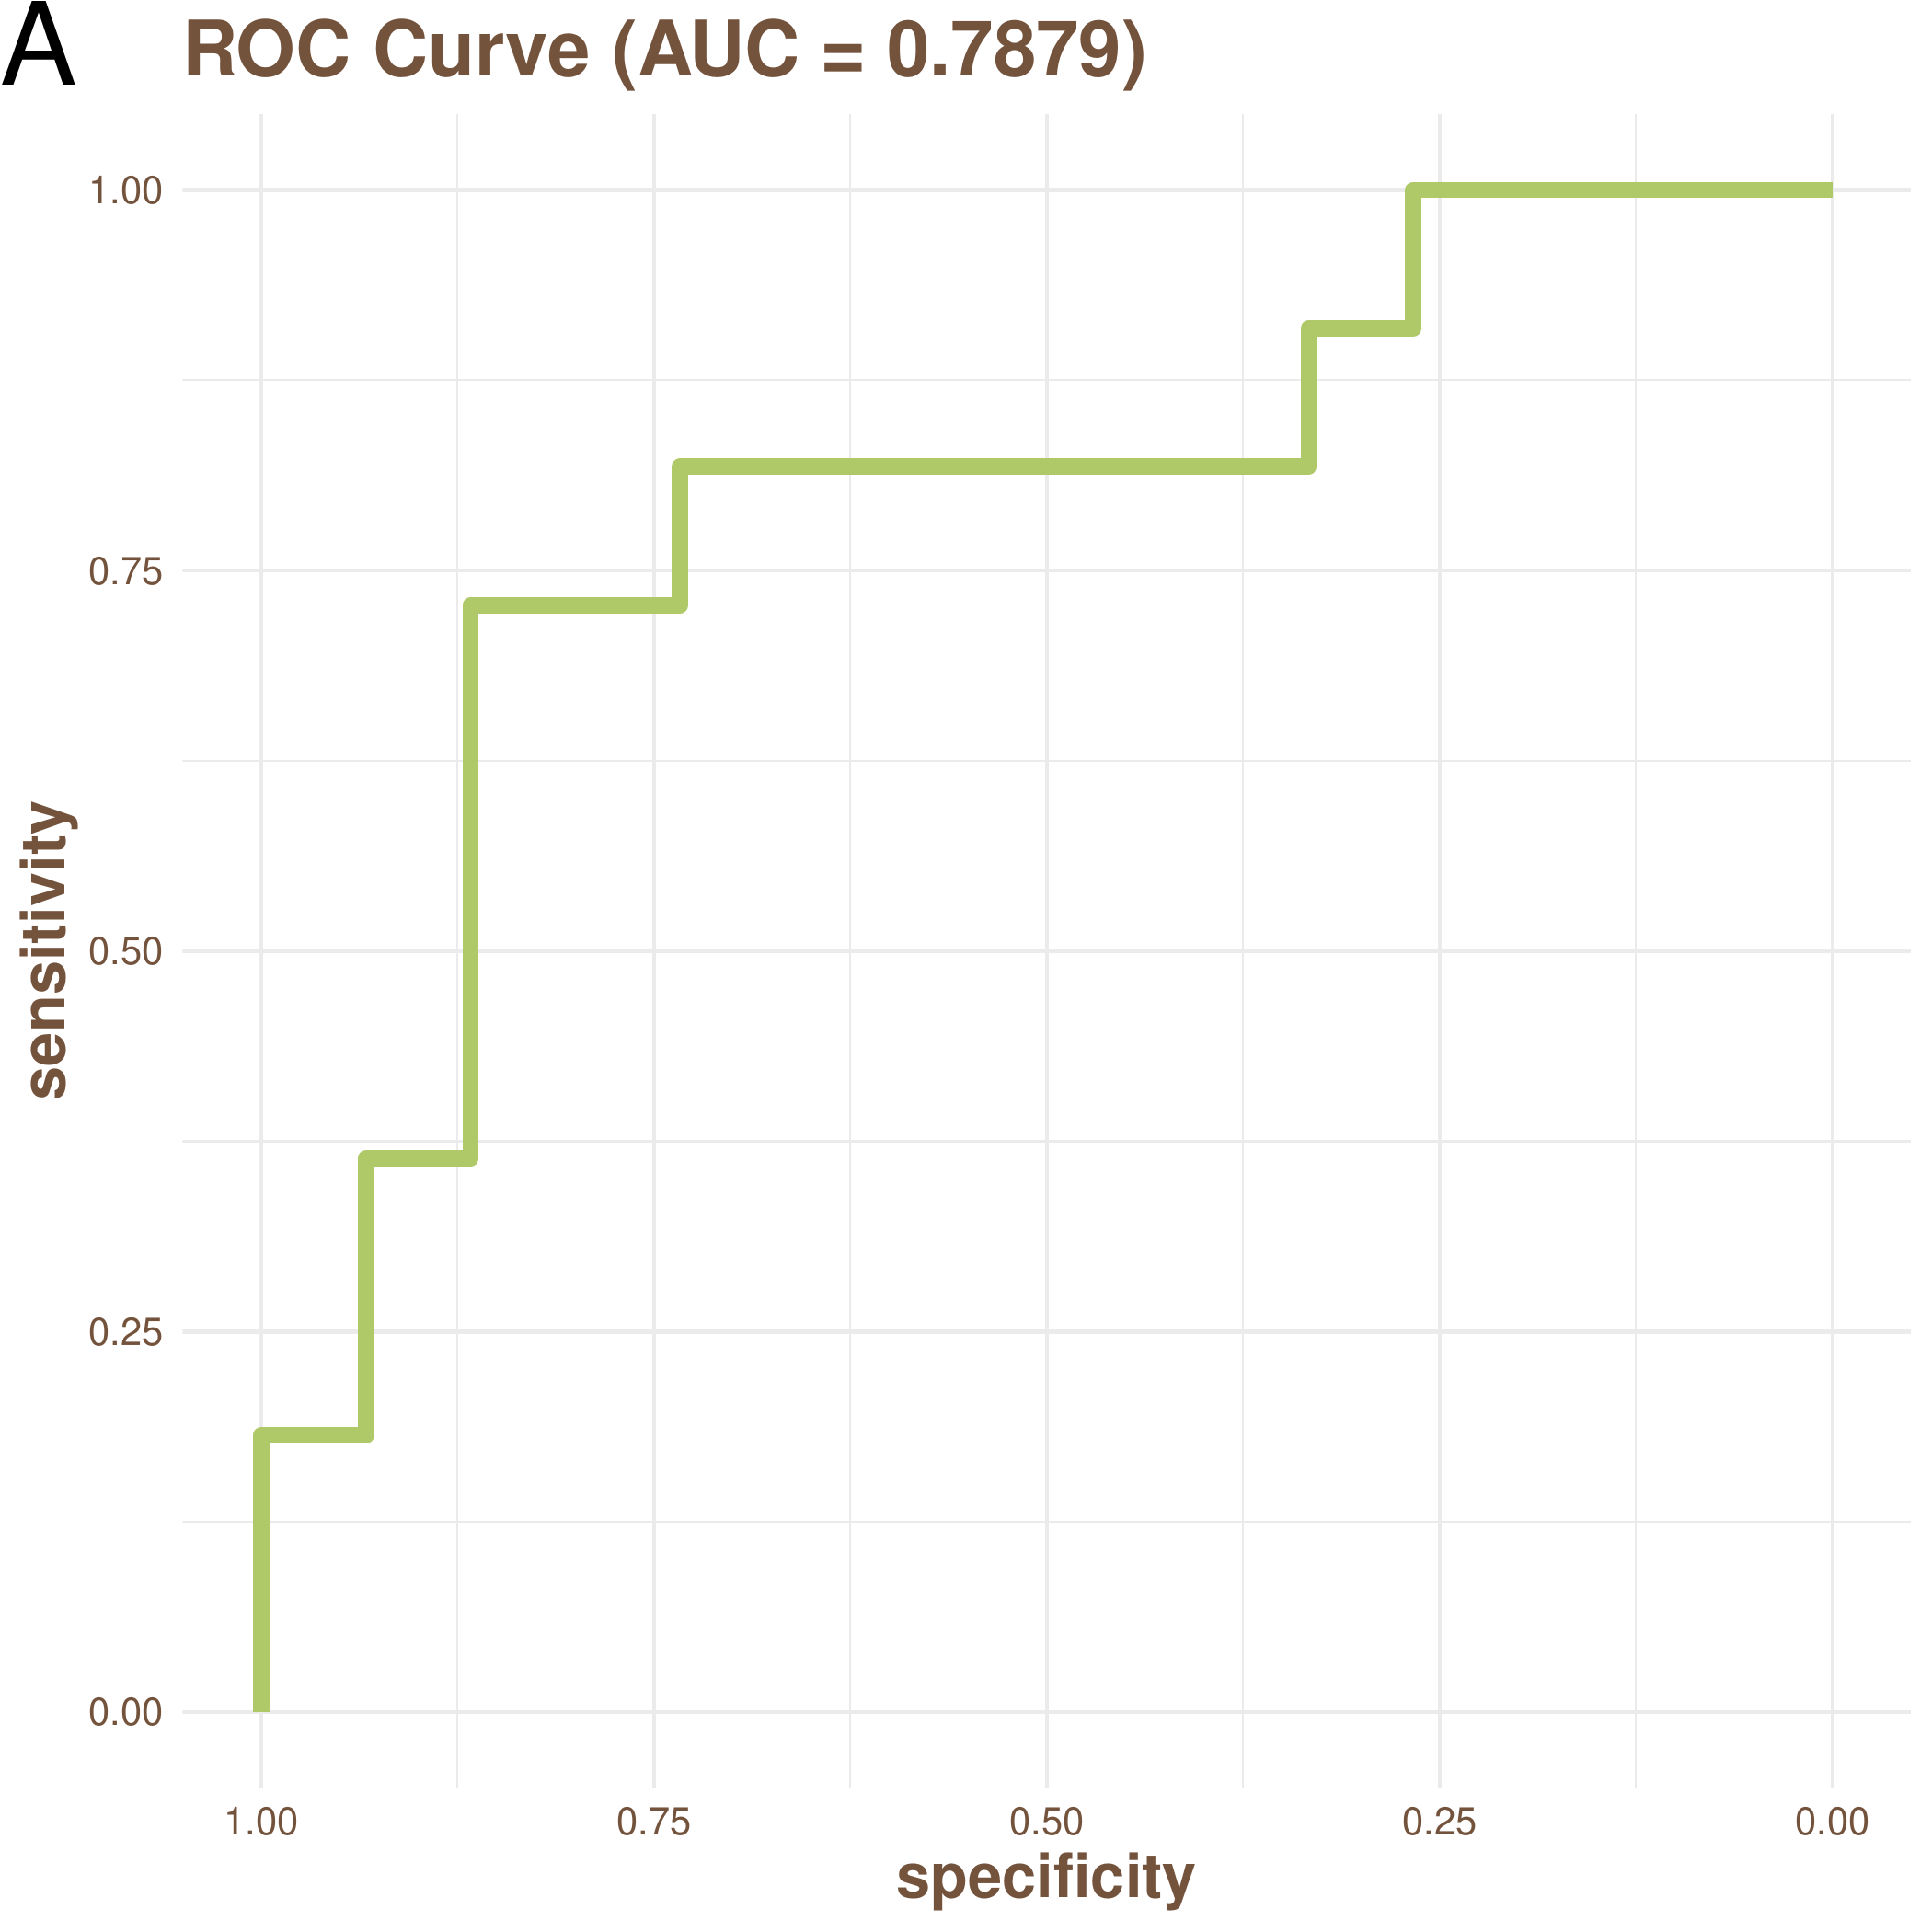
\includegraphics[width=0.5\textwidth,height=0.5\textheight]{../../Analysis_shotgun_ERP012177/03_ML/shotgun/atlas_binning/ERP012177_binning_best.model_draw_Roc_plot.png}
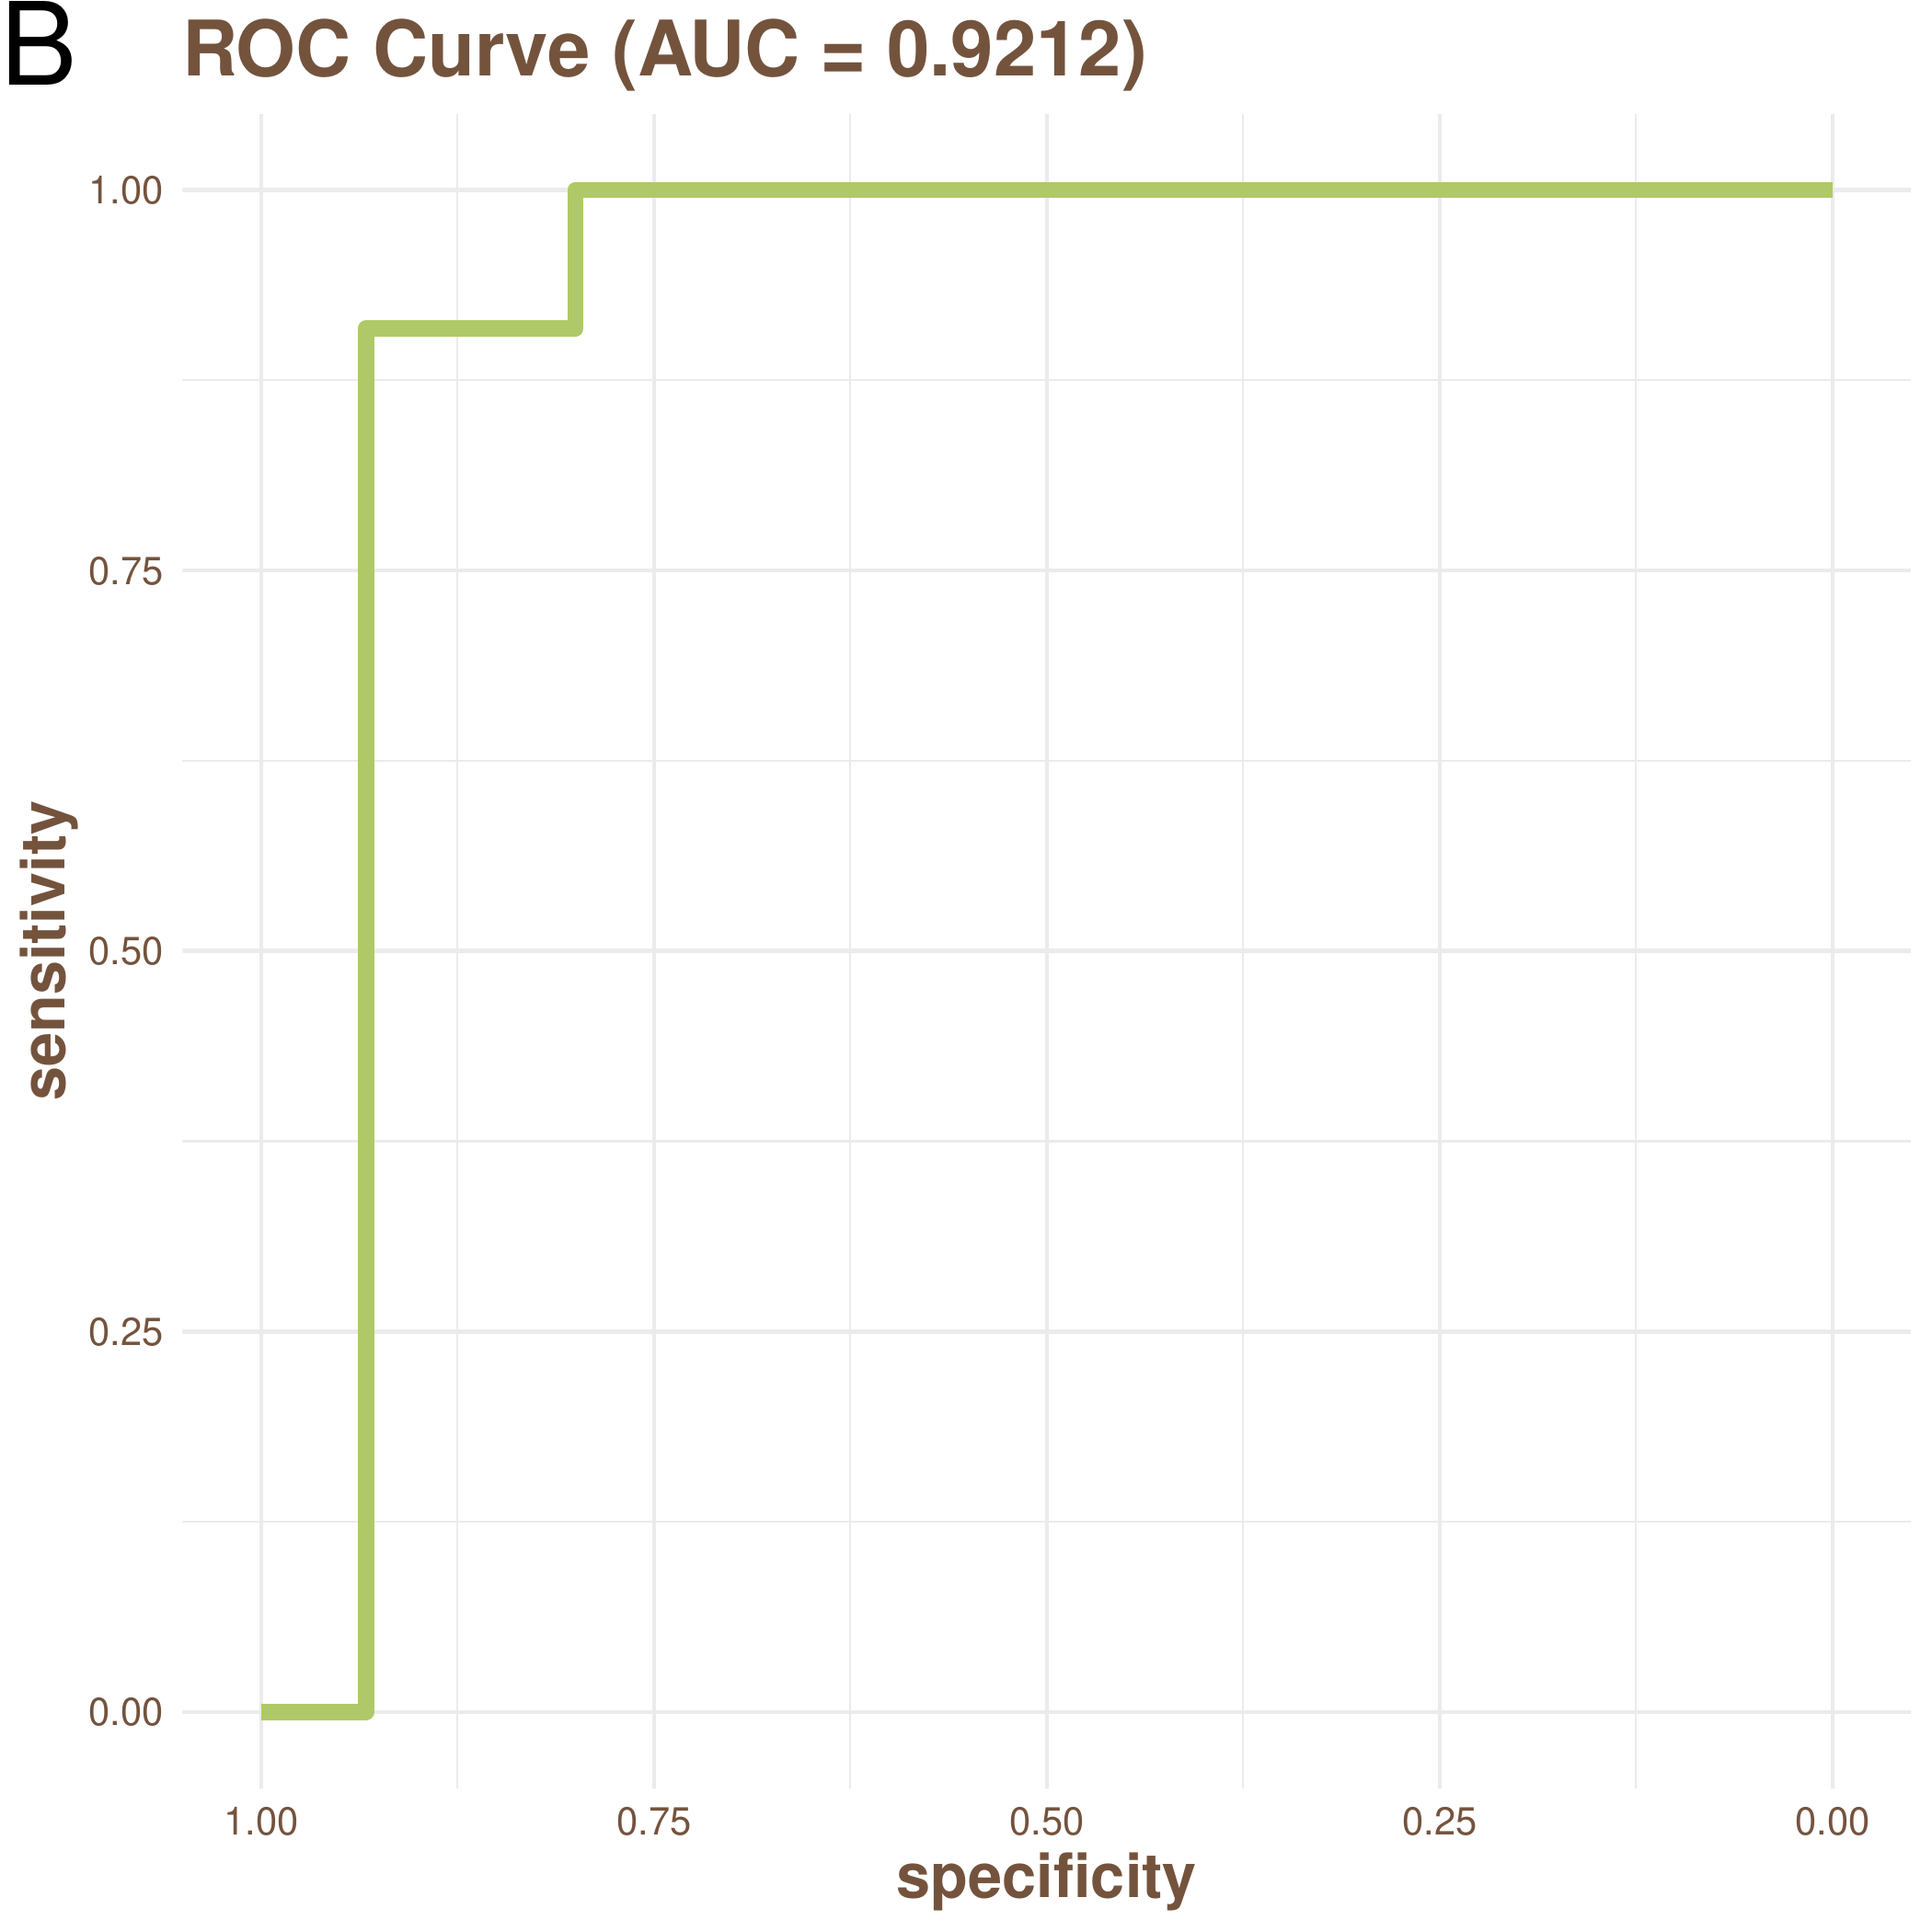
\includegraphics[width=0.5\textwidth,height=0.5\textheight]{../../Analysis_shotgun_ERP012177/03_ML/shotgun/krakens/ERP012177_best.model_draw_Roc_plot.png}

图1:ERP012177 atlas binning. 图2: ERP012177 krakens

\hypertarget{feature_importance}{%
\subsubsection{Feature\_importance}\label{feature_importance}}

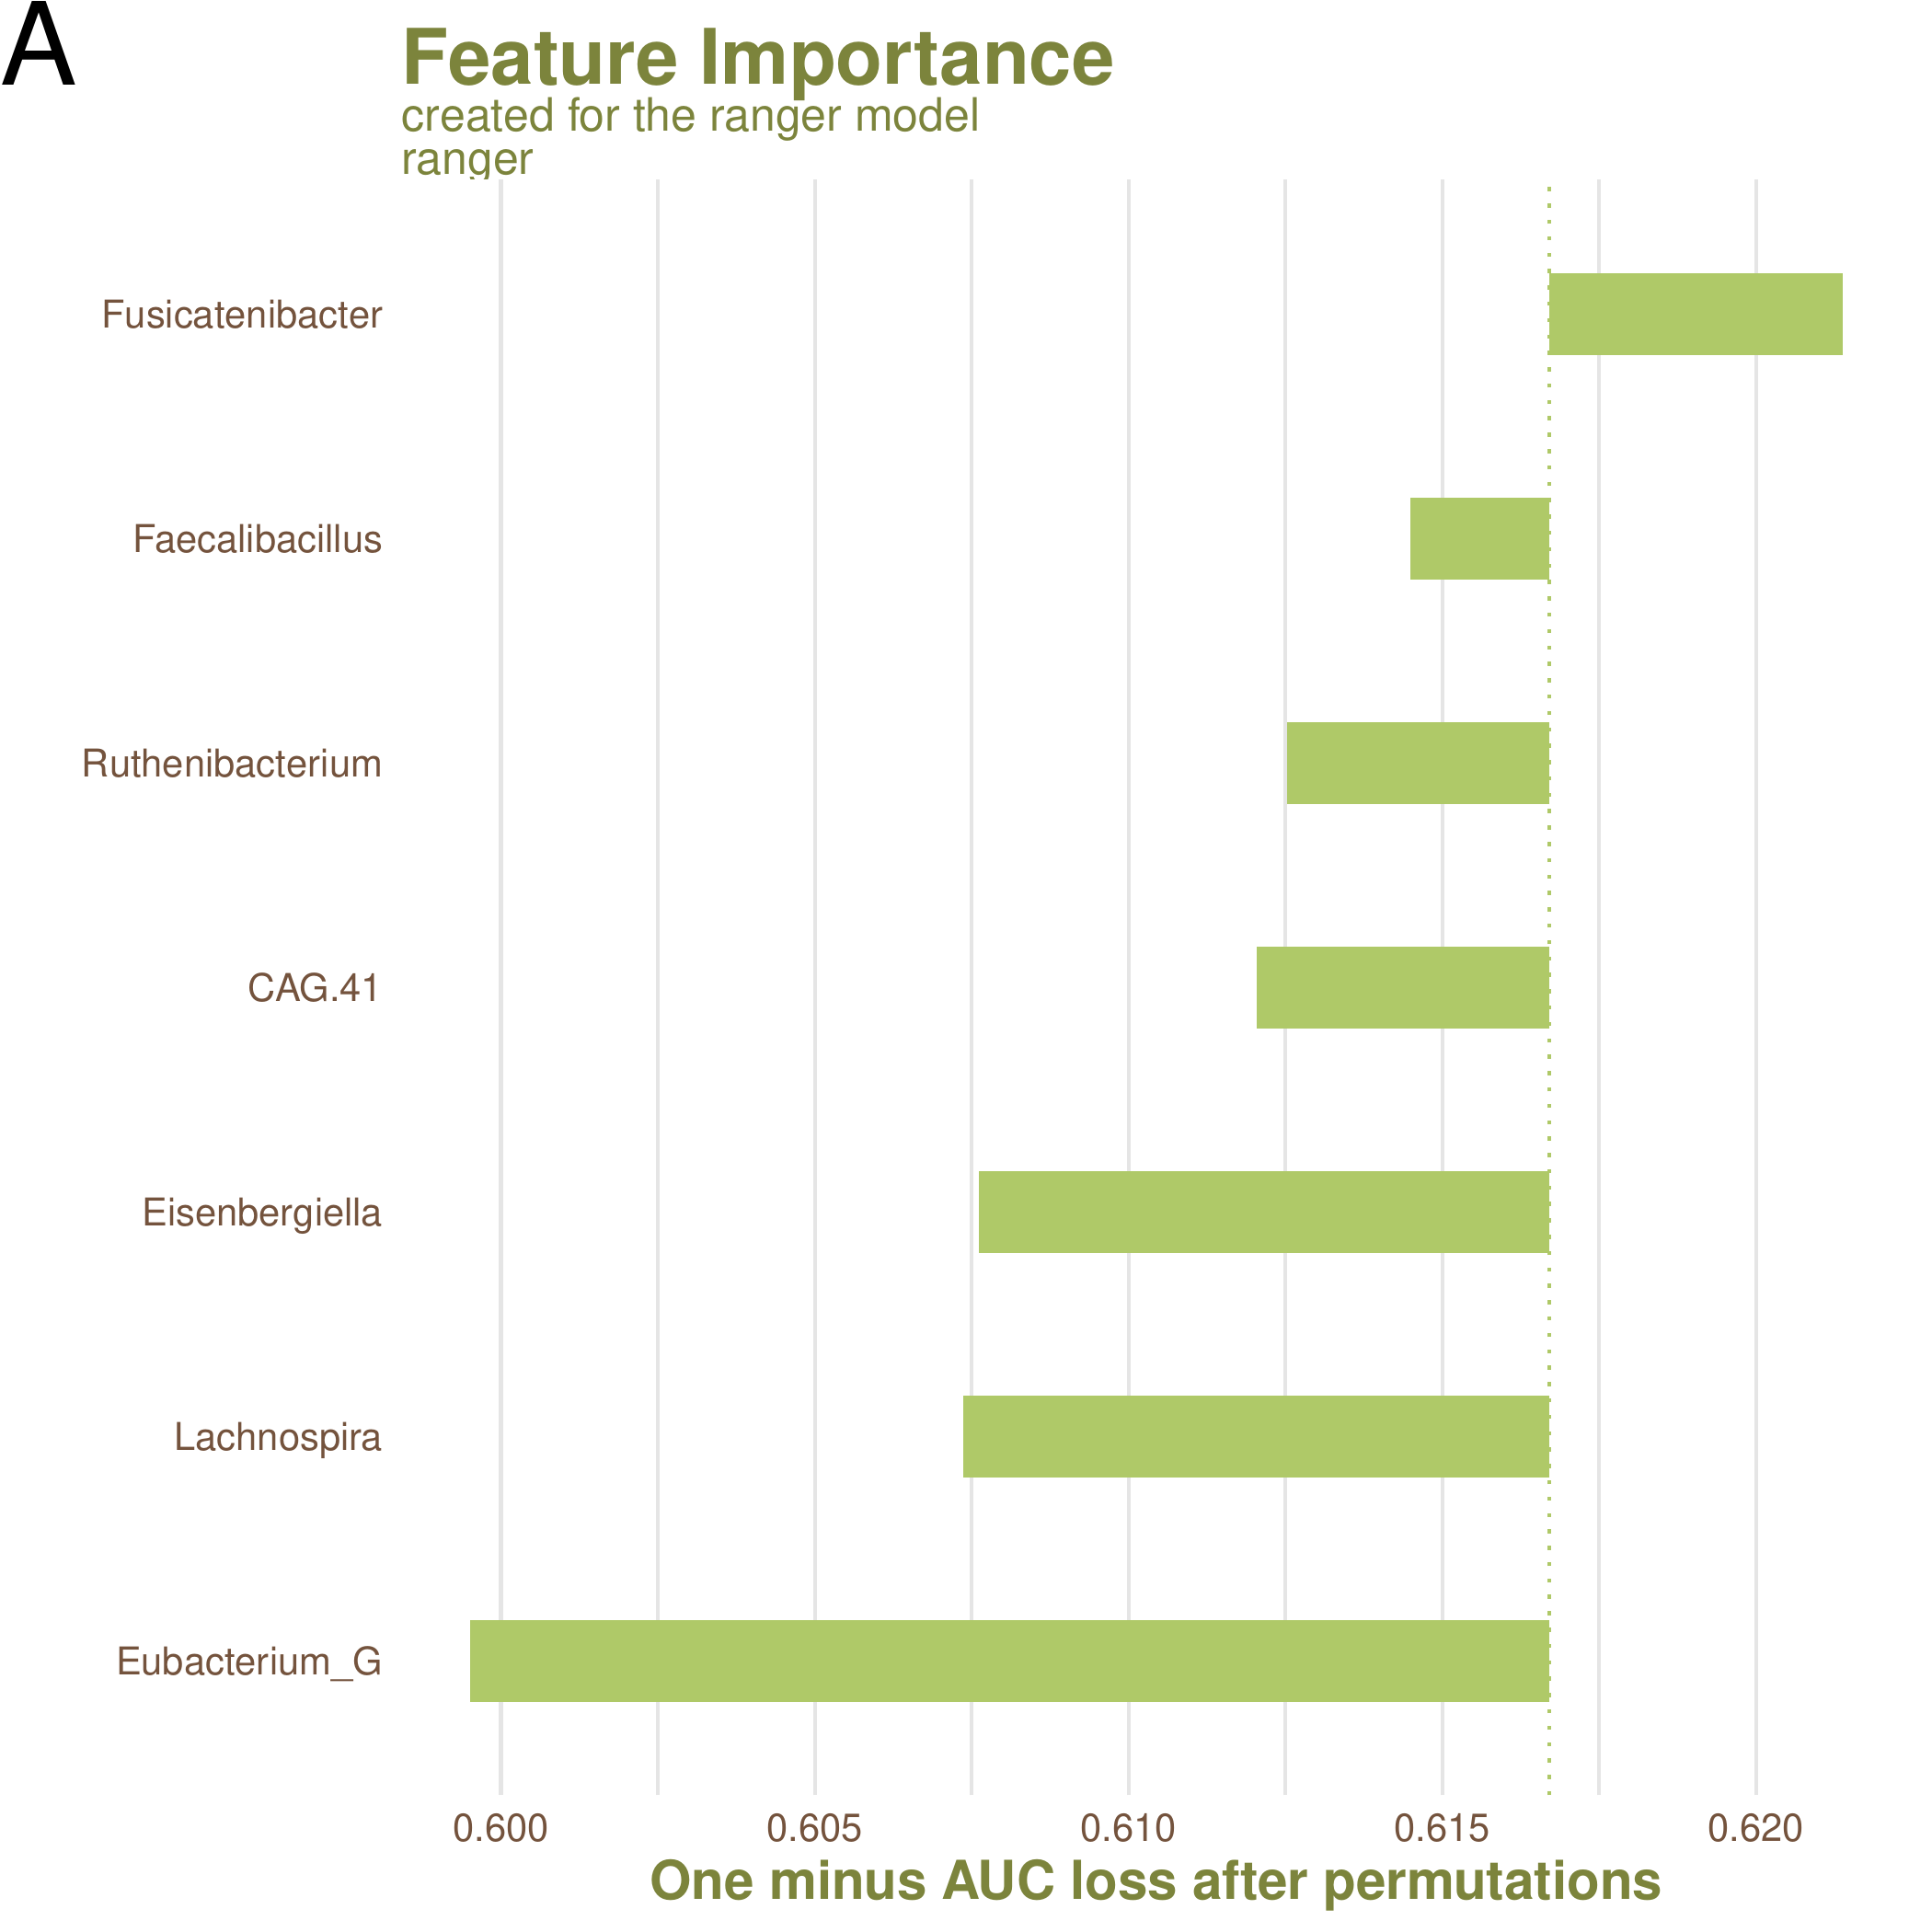
\includegraphics[width=0.5\textwidth,height=0.5\textheight]{../../Analysis_shotgun_ERP012177/03_ML/shotgun/atlas_binning/ERP012177_binning_best.model_draw_feature_importance_plot.png}
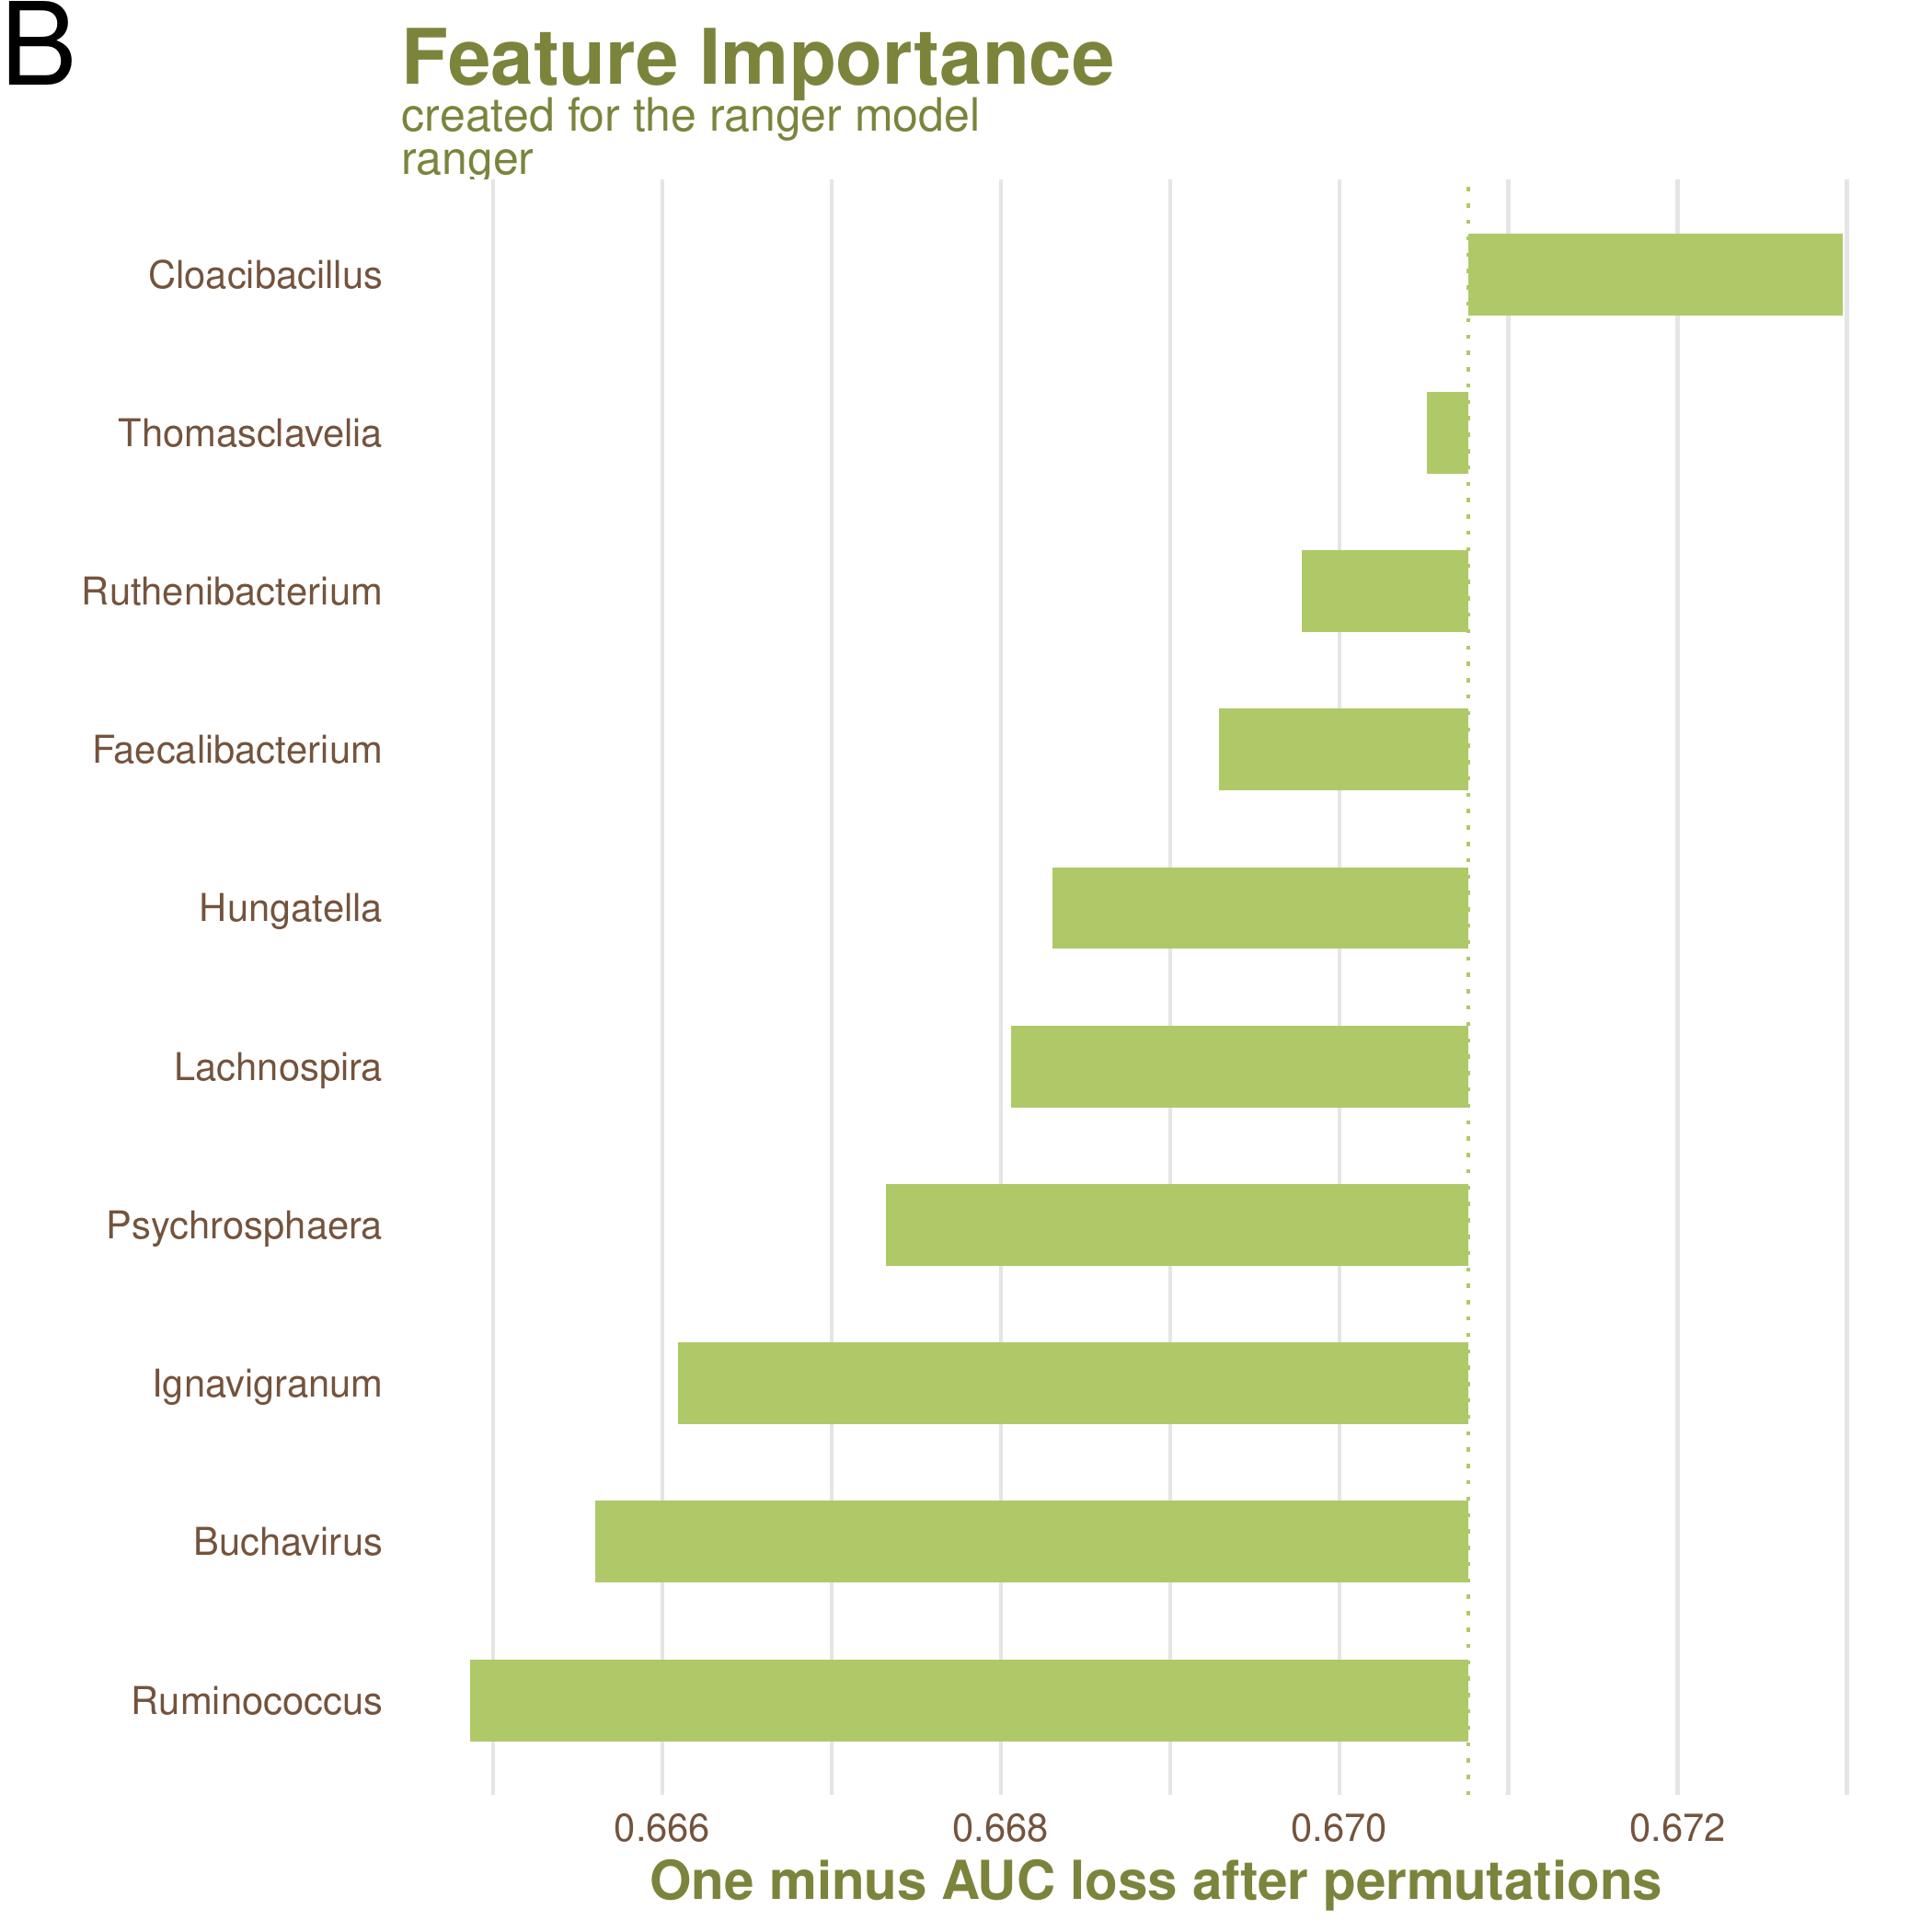
\includegraphics[width=0.5\textwidth,height=0.5\textheight]{../../Analysis_shotgun_ERP012177/03_ML/shotgun/krakens/ERP012177_best.model_draw_feature_importance_plot.png}

图1:ERP012177 atlas binning. 图2: ERP012177 krakens

\hypertarget{prjdb4176}{%
\subsection{PRJDB4176}\label{prjdb4176}}

\hypertarget{roc-1}{%
\subsubsection{ROC}\label{roc-1}}

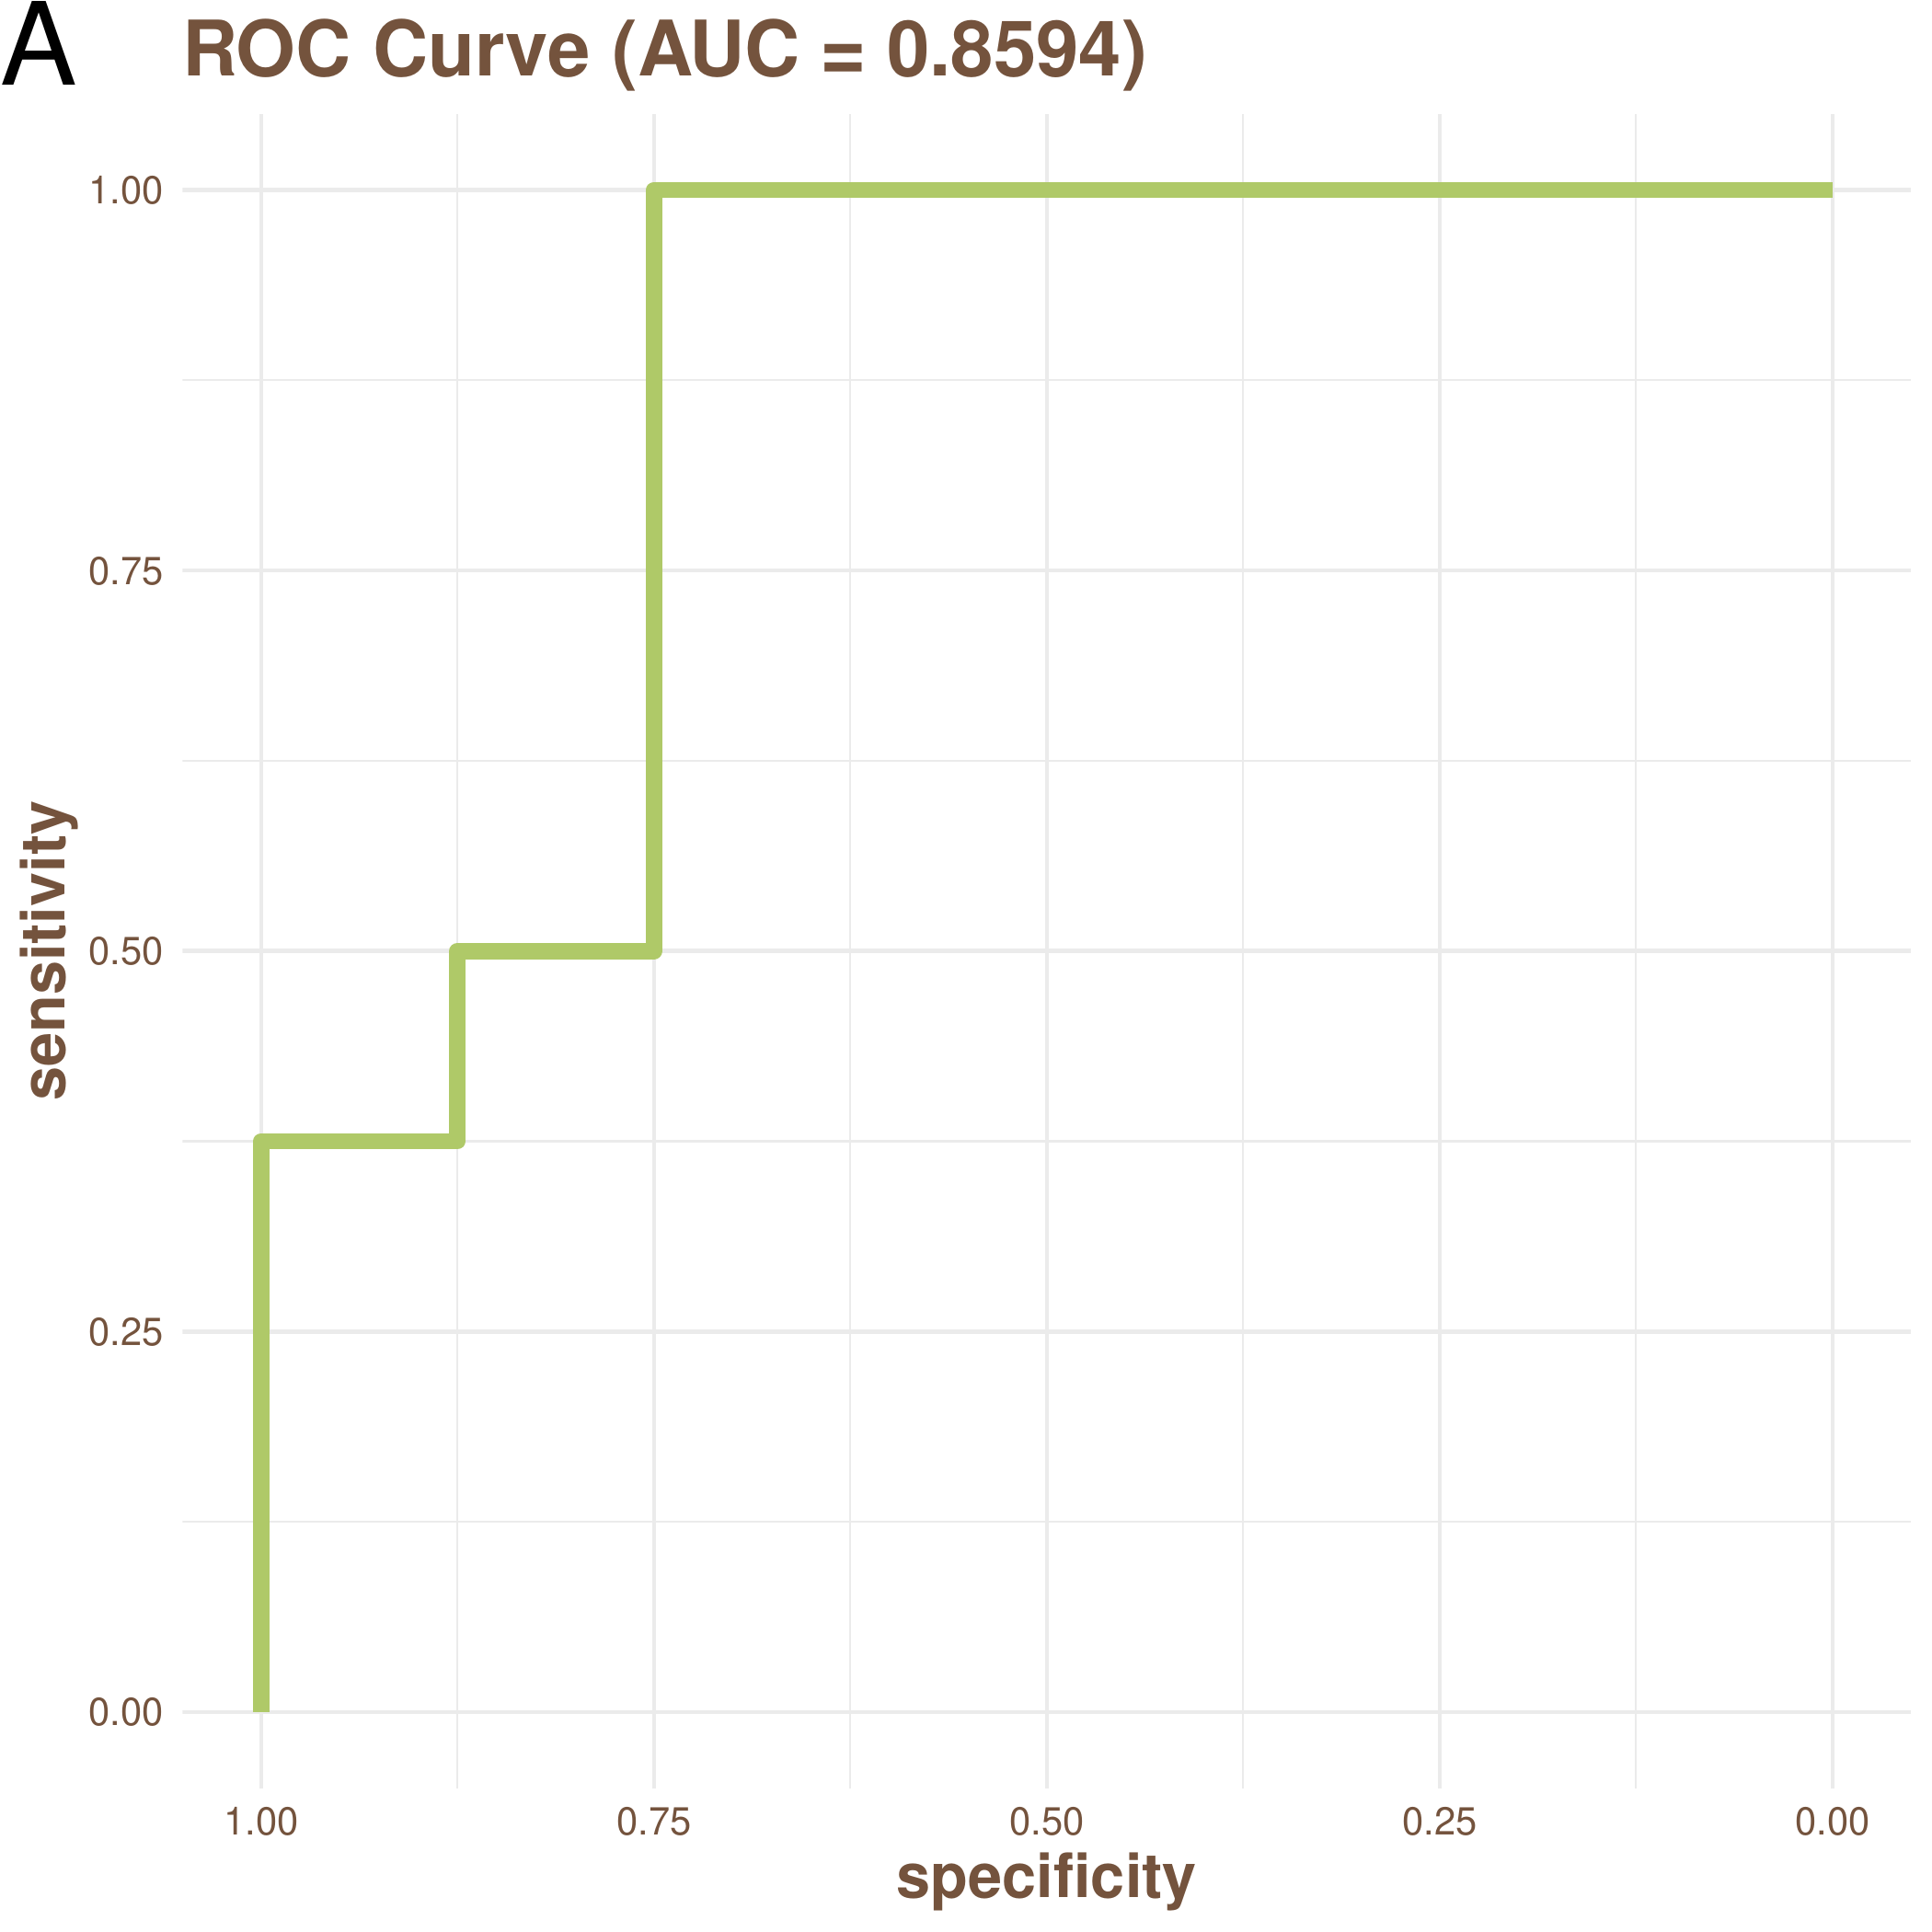
\includegraphics[width=0.5\textwidth,height=0.5\textheight]{../../Analysis_shotgun_PRJDB4176/03_ML/shotgun/atlas_binning/PRJDB4176_binning_best.model_draw_Roc_plot.png}
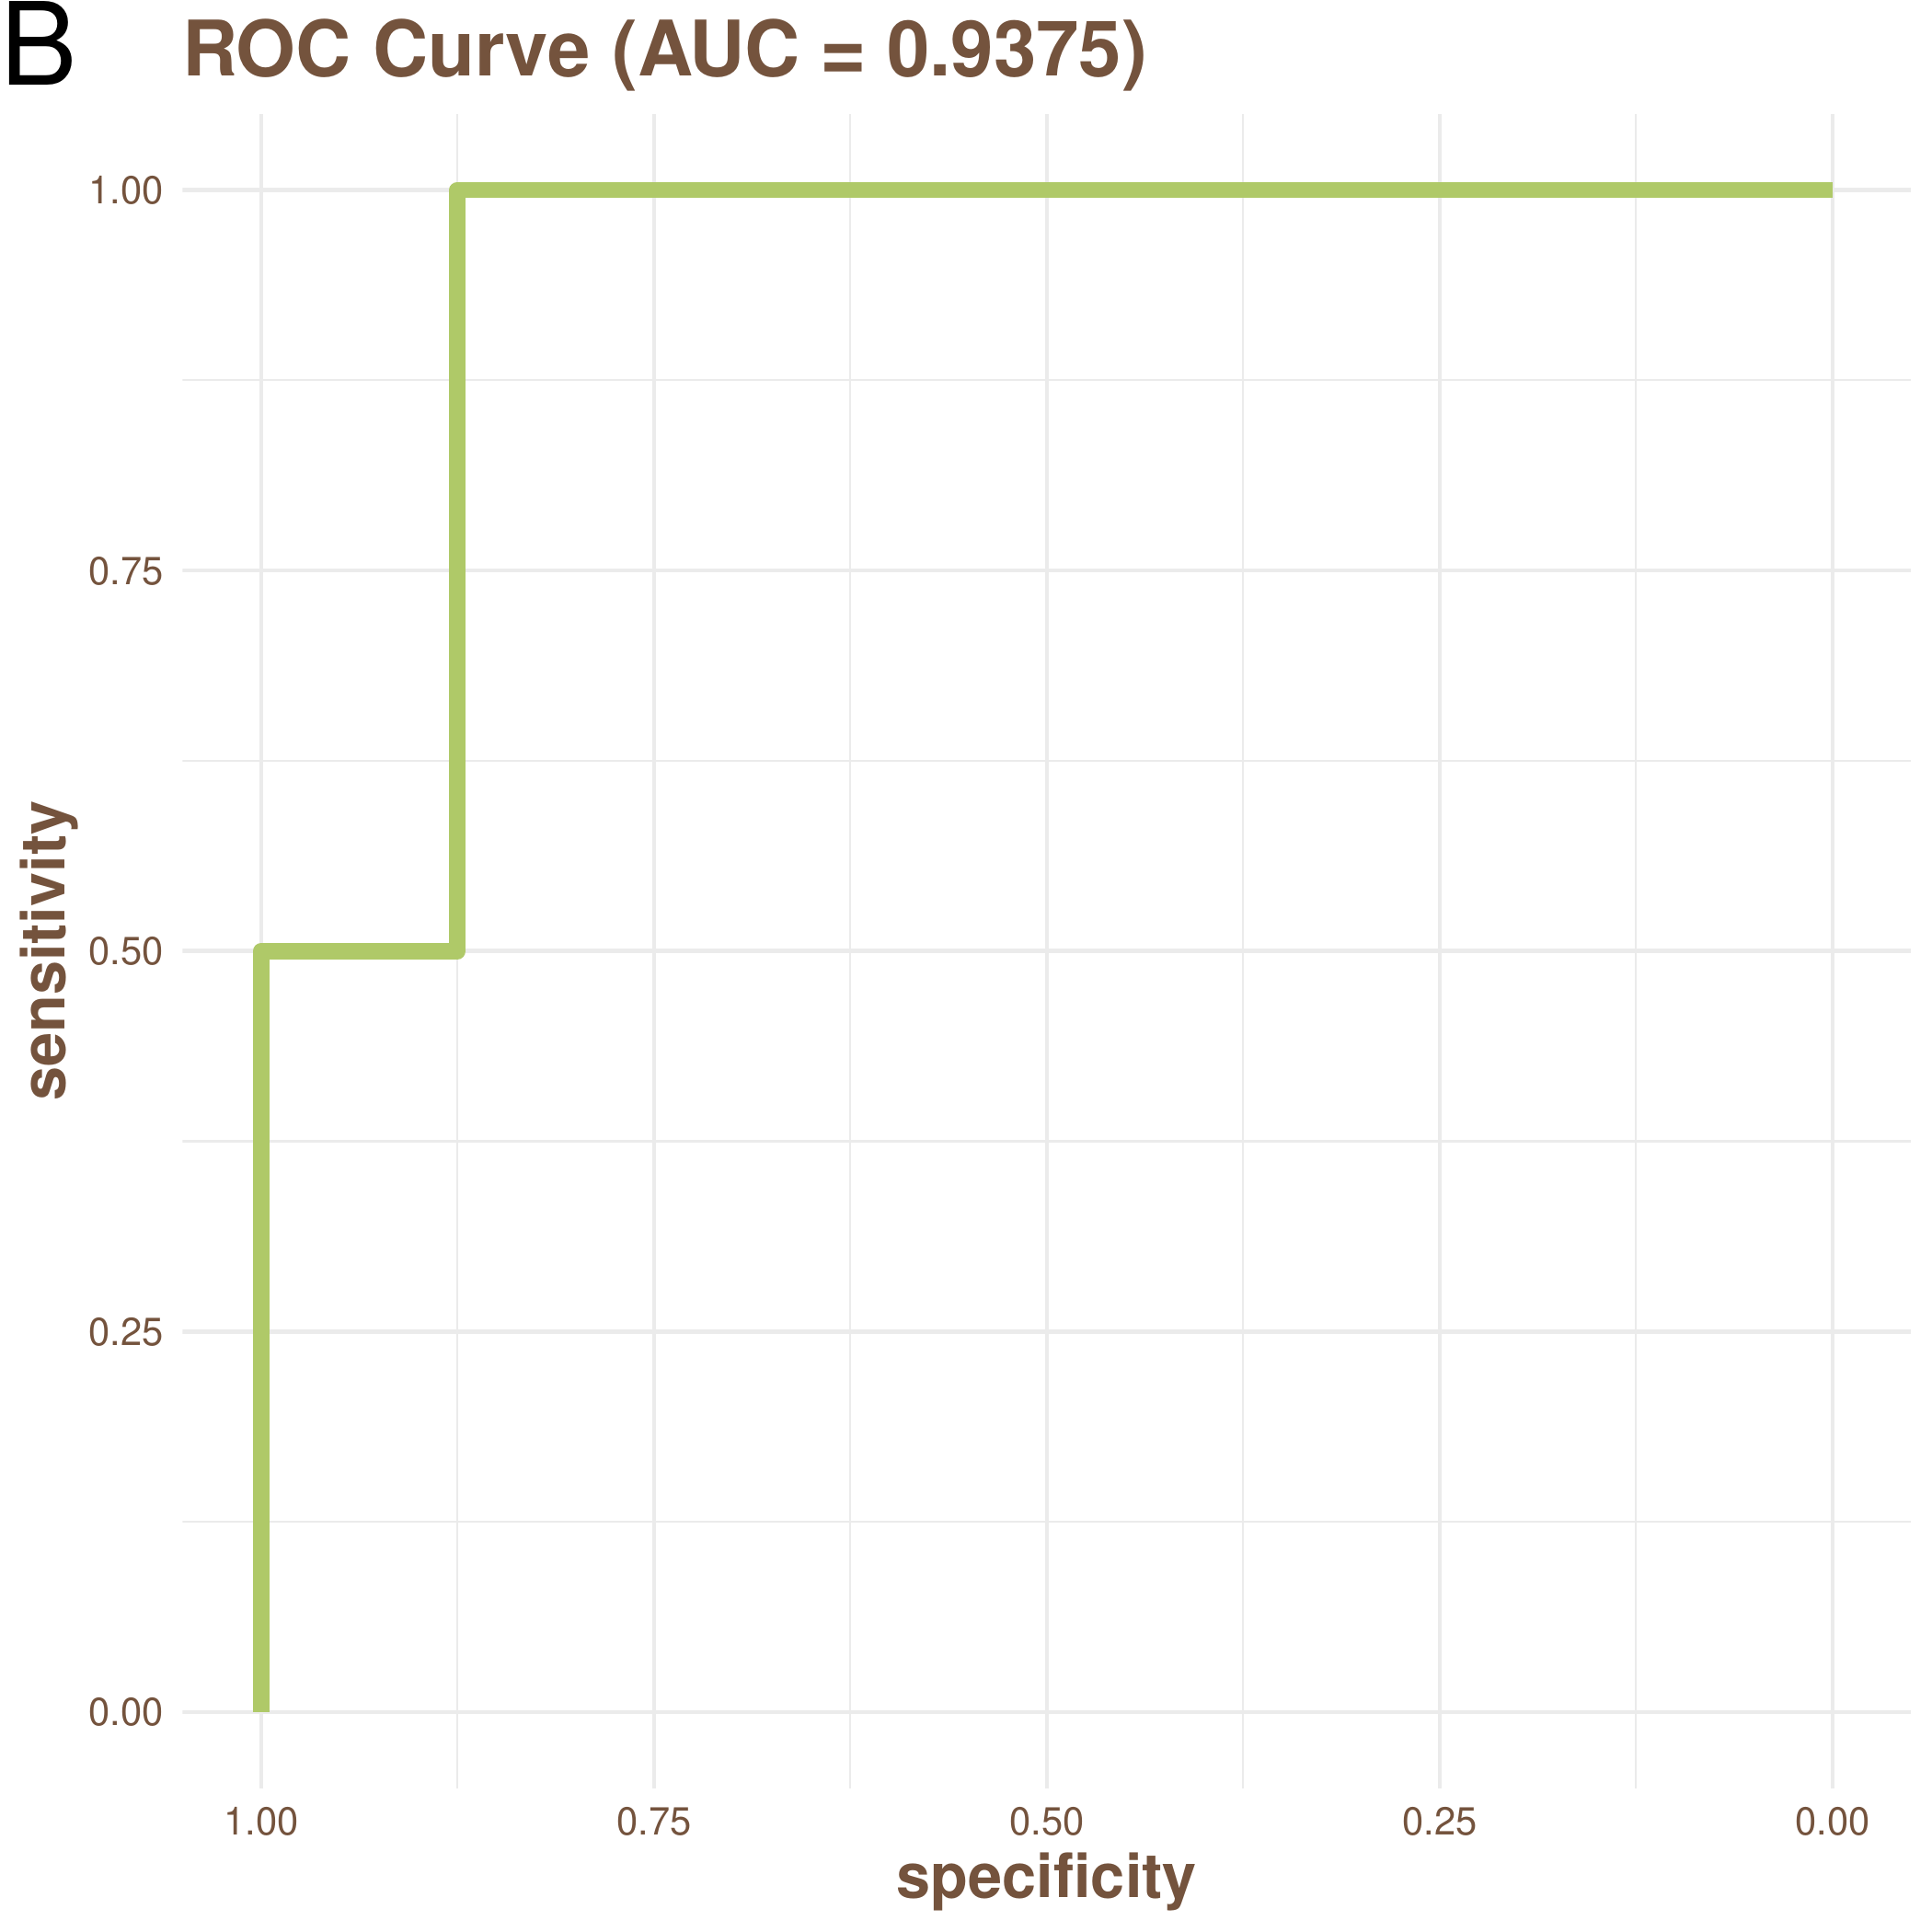
\includegraphics[width=0.5\textwidth,height=0.5\textheight]{../../Analysis_shotgun_PRJDB4176/03_ML/shotgun/krakens/PRJDB4176_best.model_draw_Roc_plot.png}

\hypertarget{feature_importance-1}{%
\subsubsection{Feature\_importance}\label{feature_importance-1}}

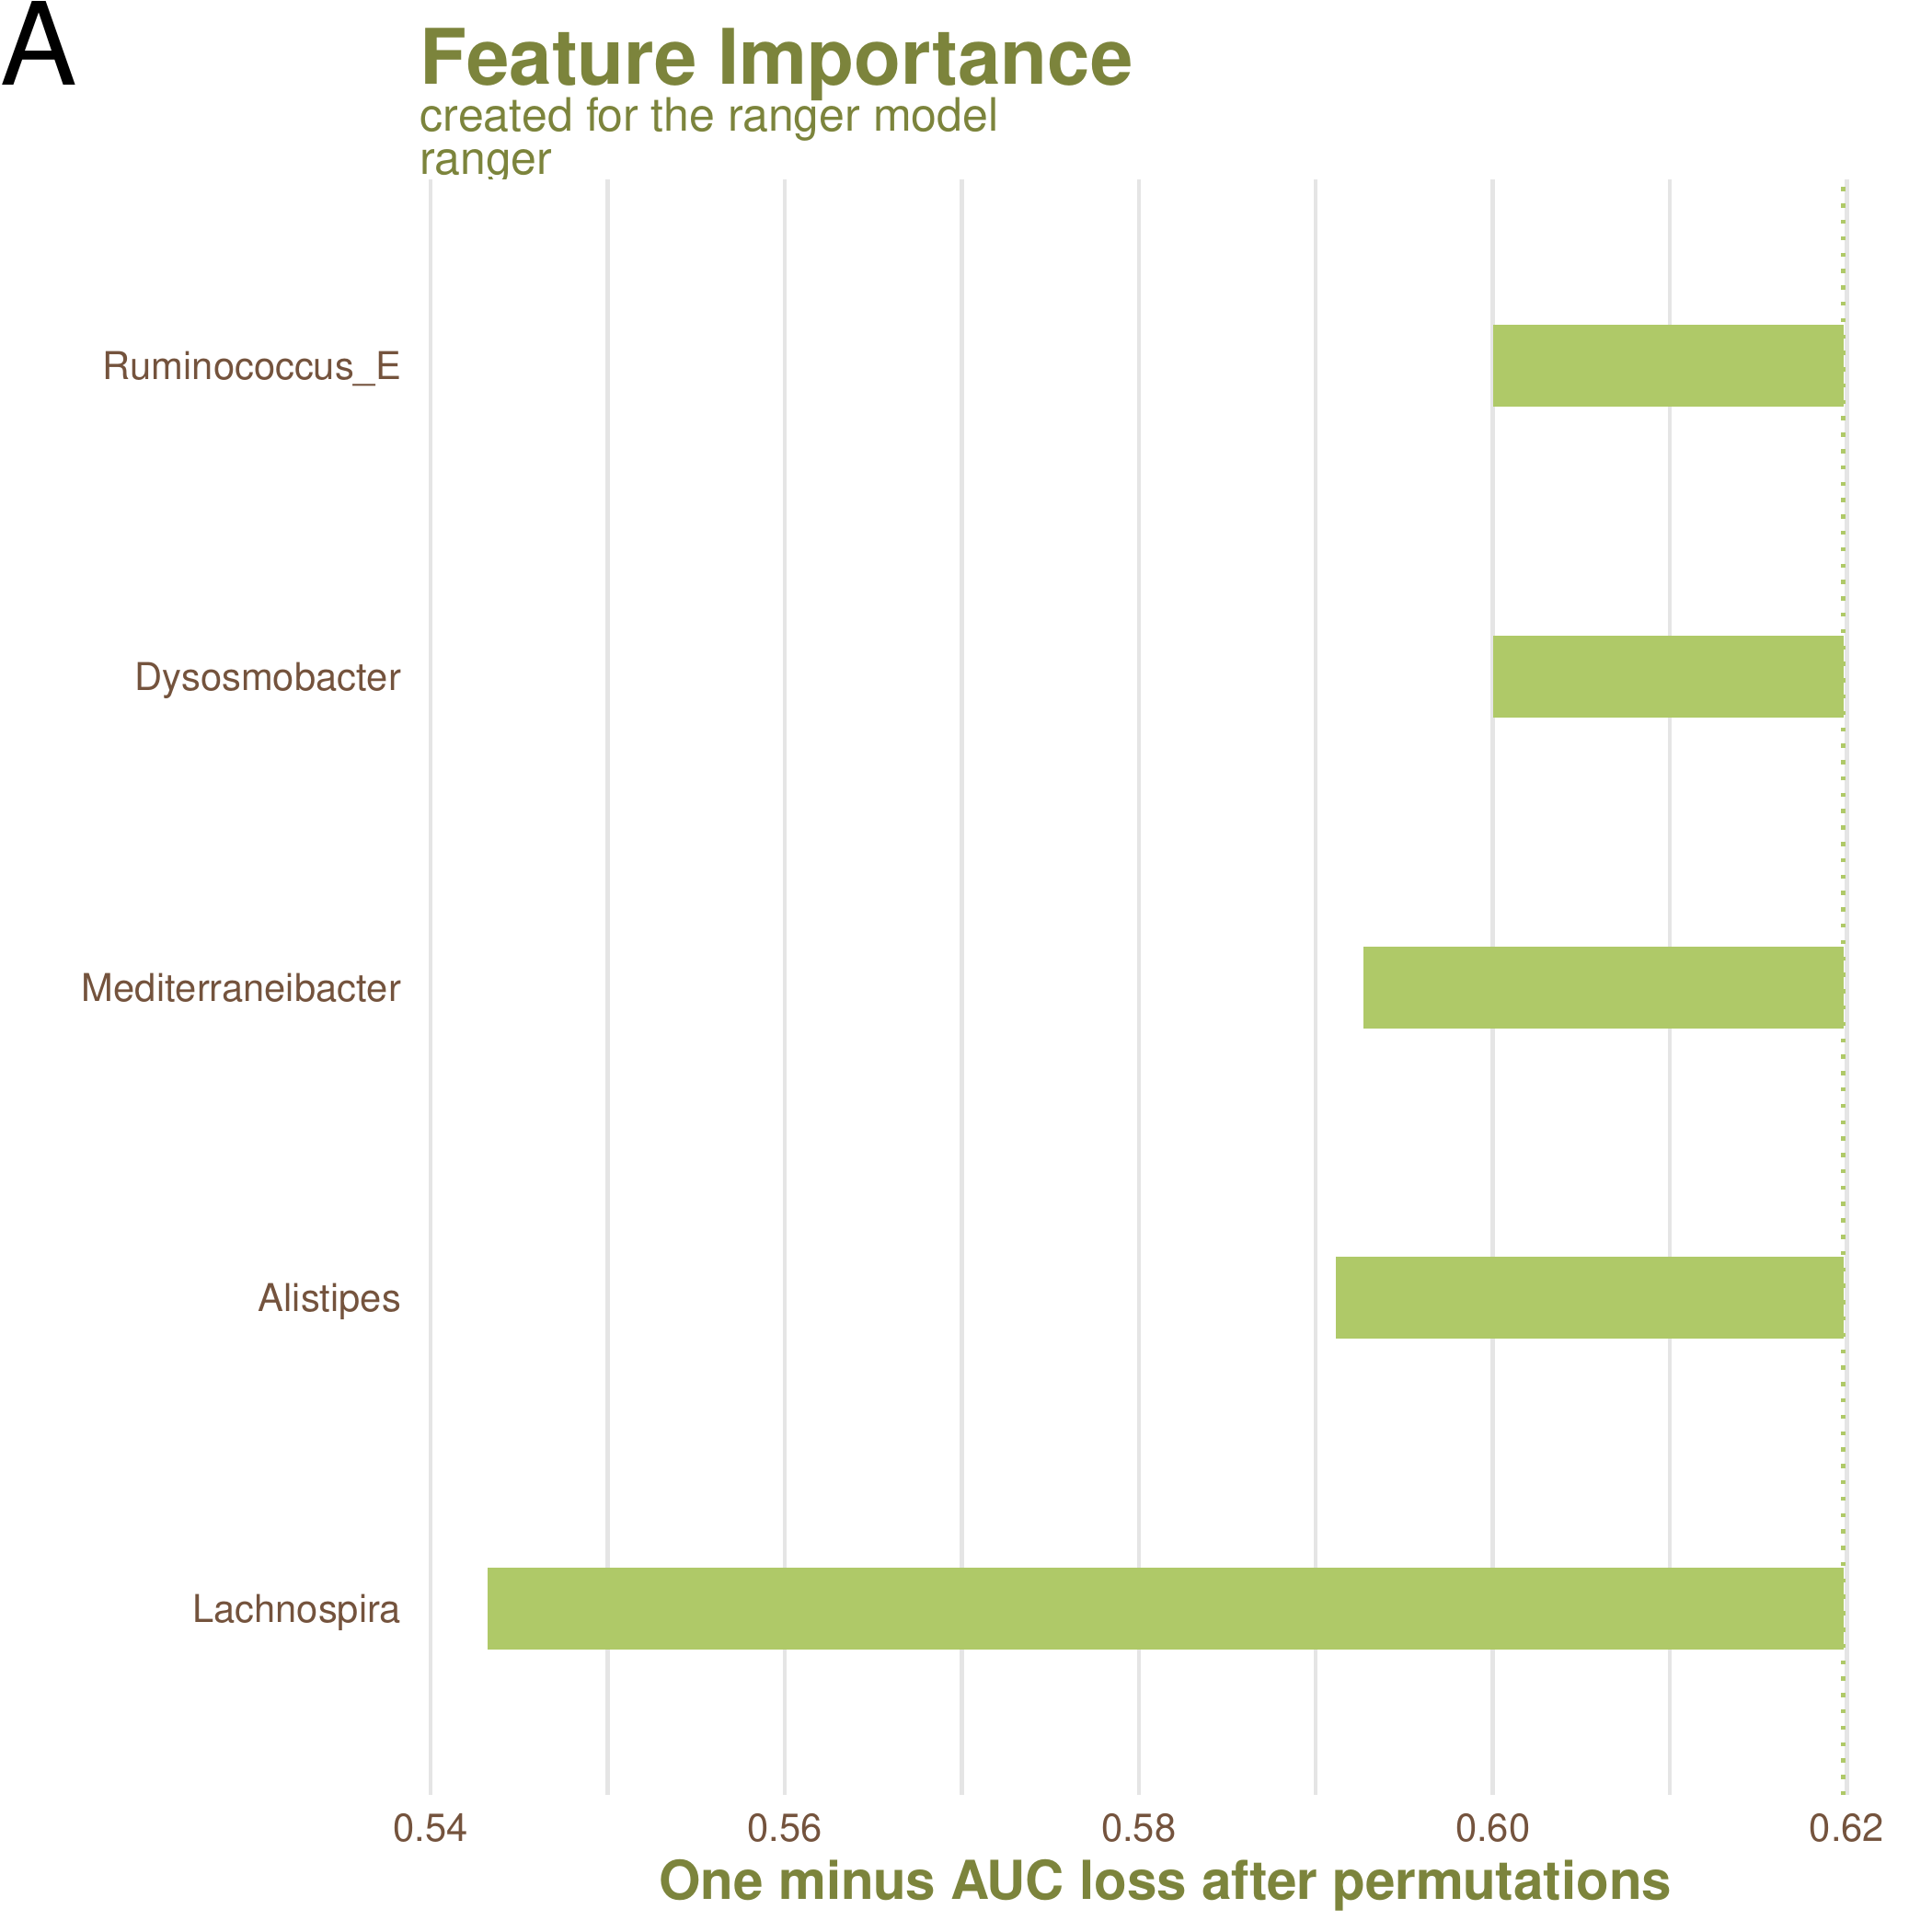
\includegraphics[width=0.5\textwidth,height=0.5\textheight]{../../Analysis_shotgun_PRJDB4176/03_ML/shotgun/atlas_binning/PRJDB4176_binning_best.model_draw_feature_importance_plot.png}
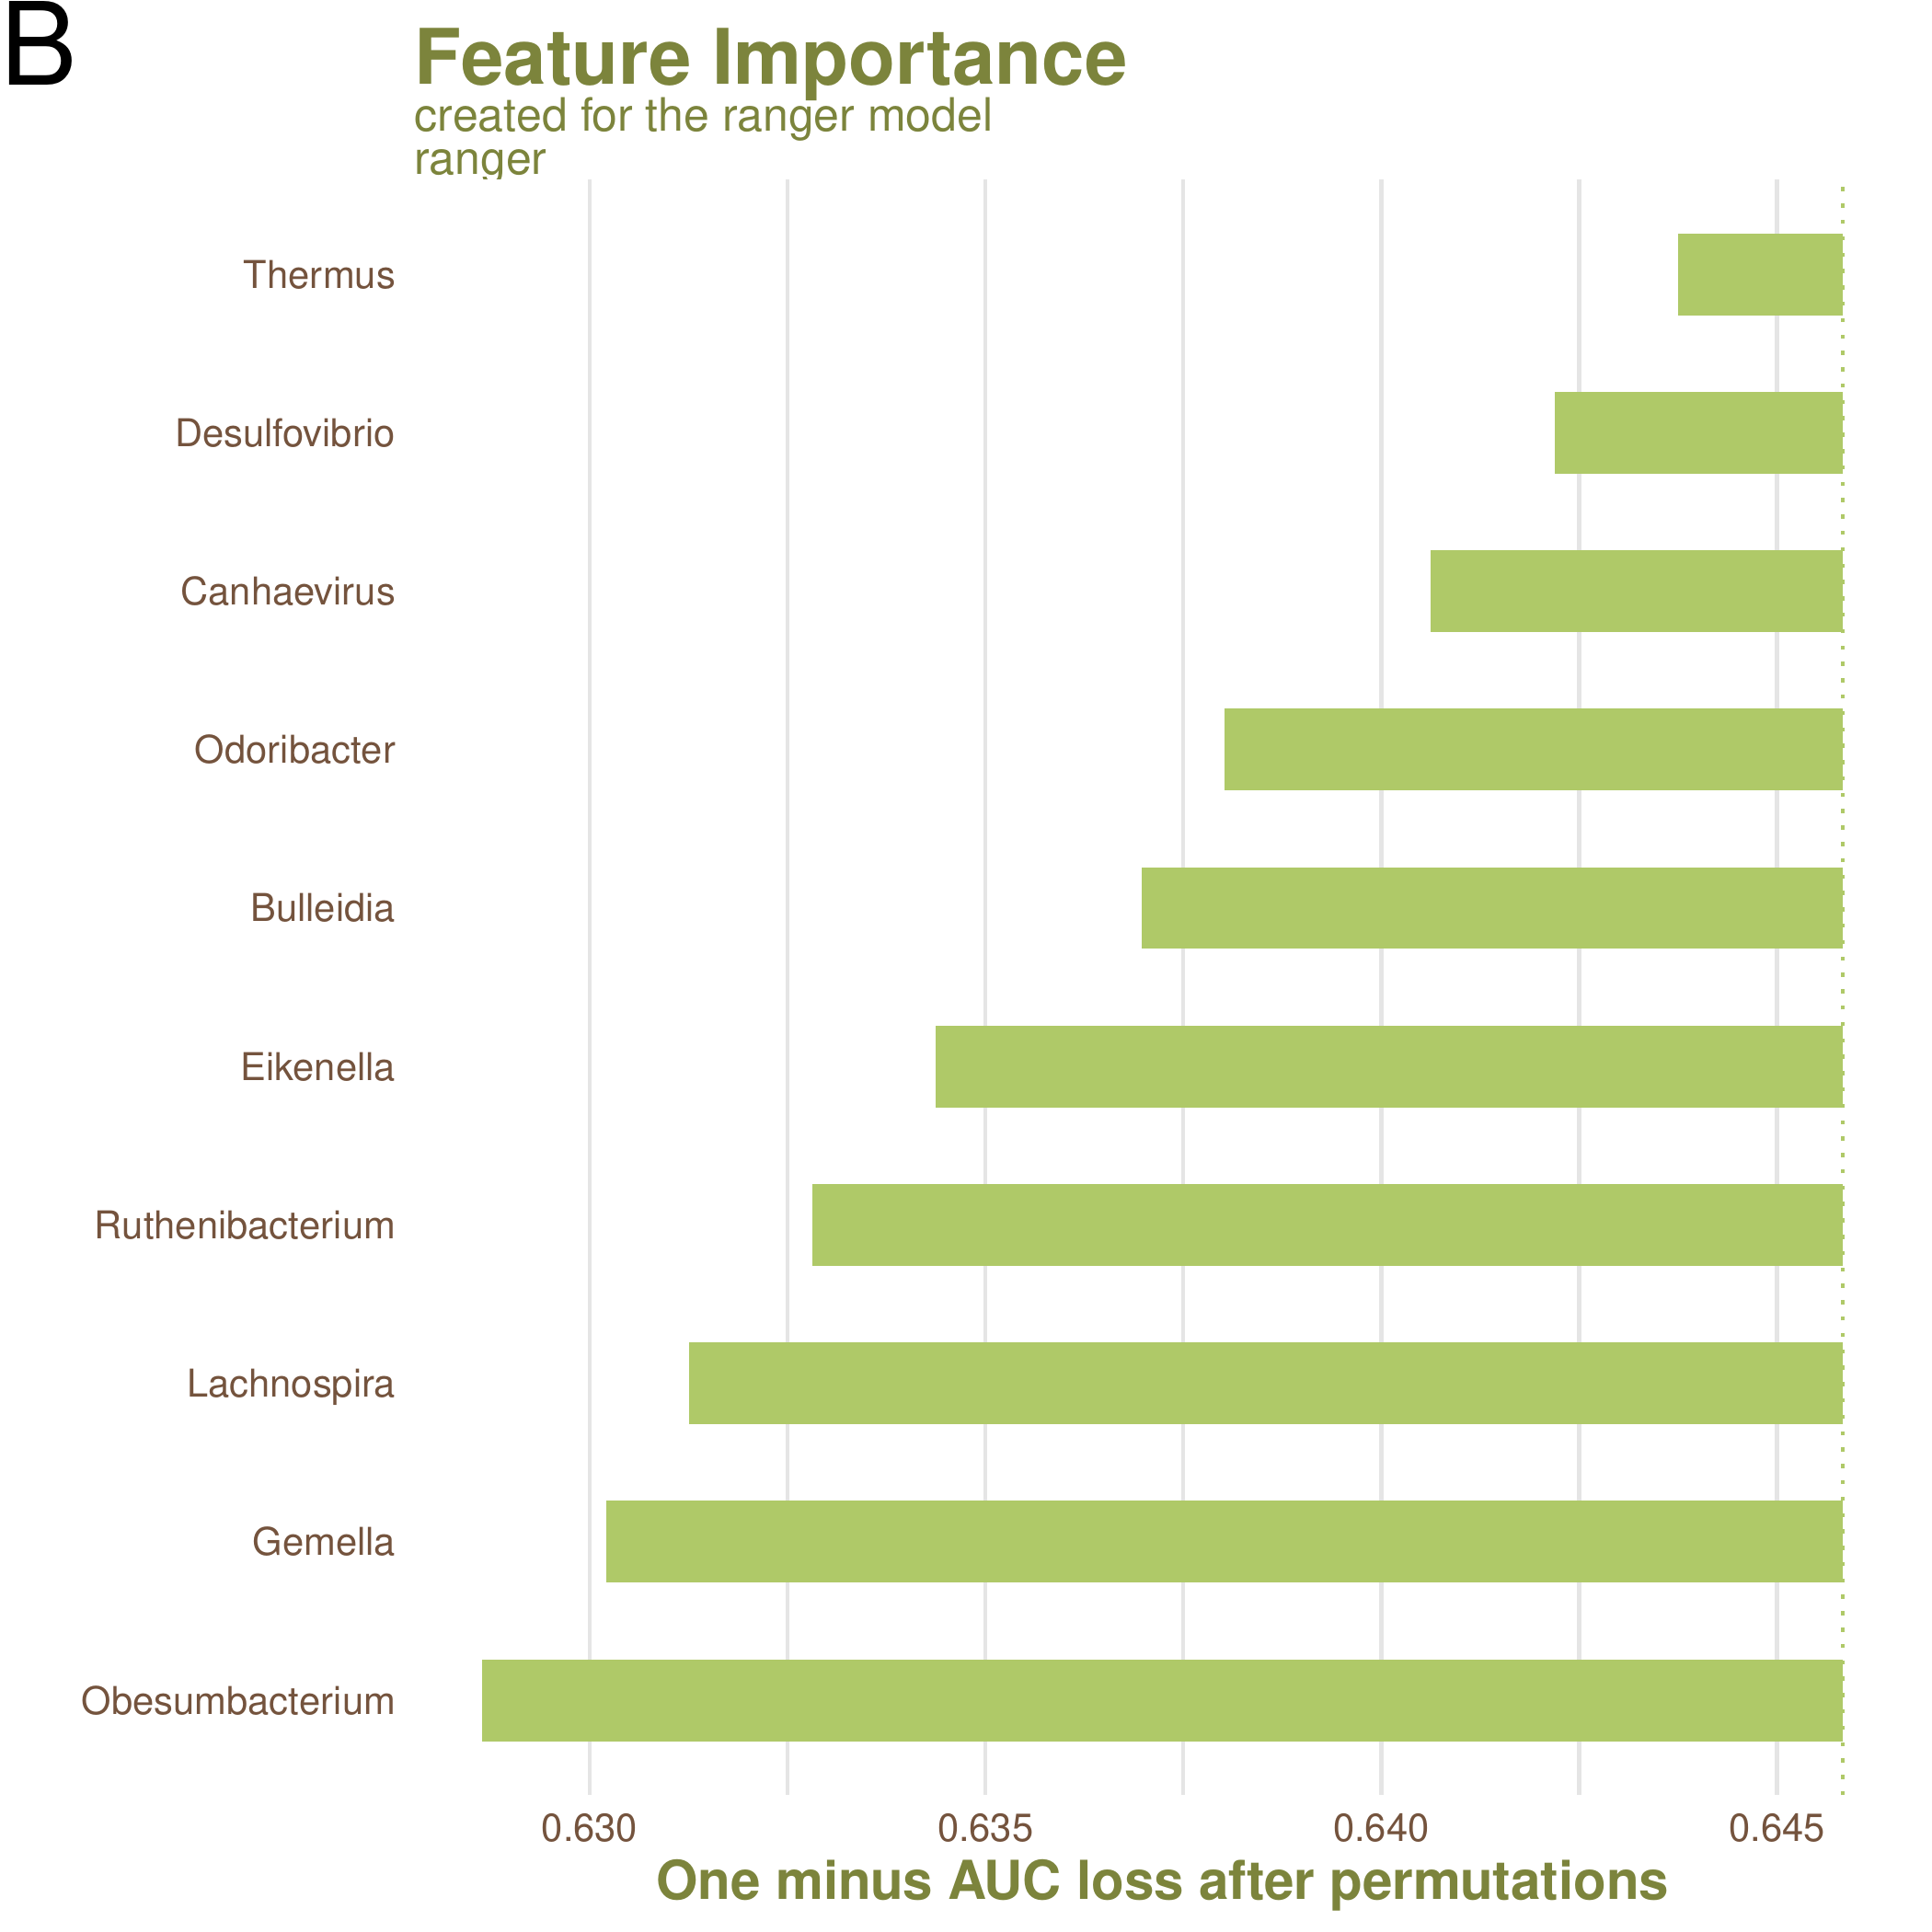
\includegraphics[width=0.5\textwidth,height=0.5\textheight]{../../Analysis_shotgun_PRJDB4176/03_ML/shotgun/krakens/PRJDB4176_best.model_draw_feature_importance_plot.png}

\hypertarget{figure3-wilcoxon}{%
\section{Figure3 Wilcoxon}\label{figure3-wilcoxon}}

\hypertarget{erp012177-1}{%
\subsection{ERP012177}\label{erp012177-1}}

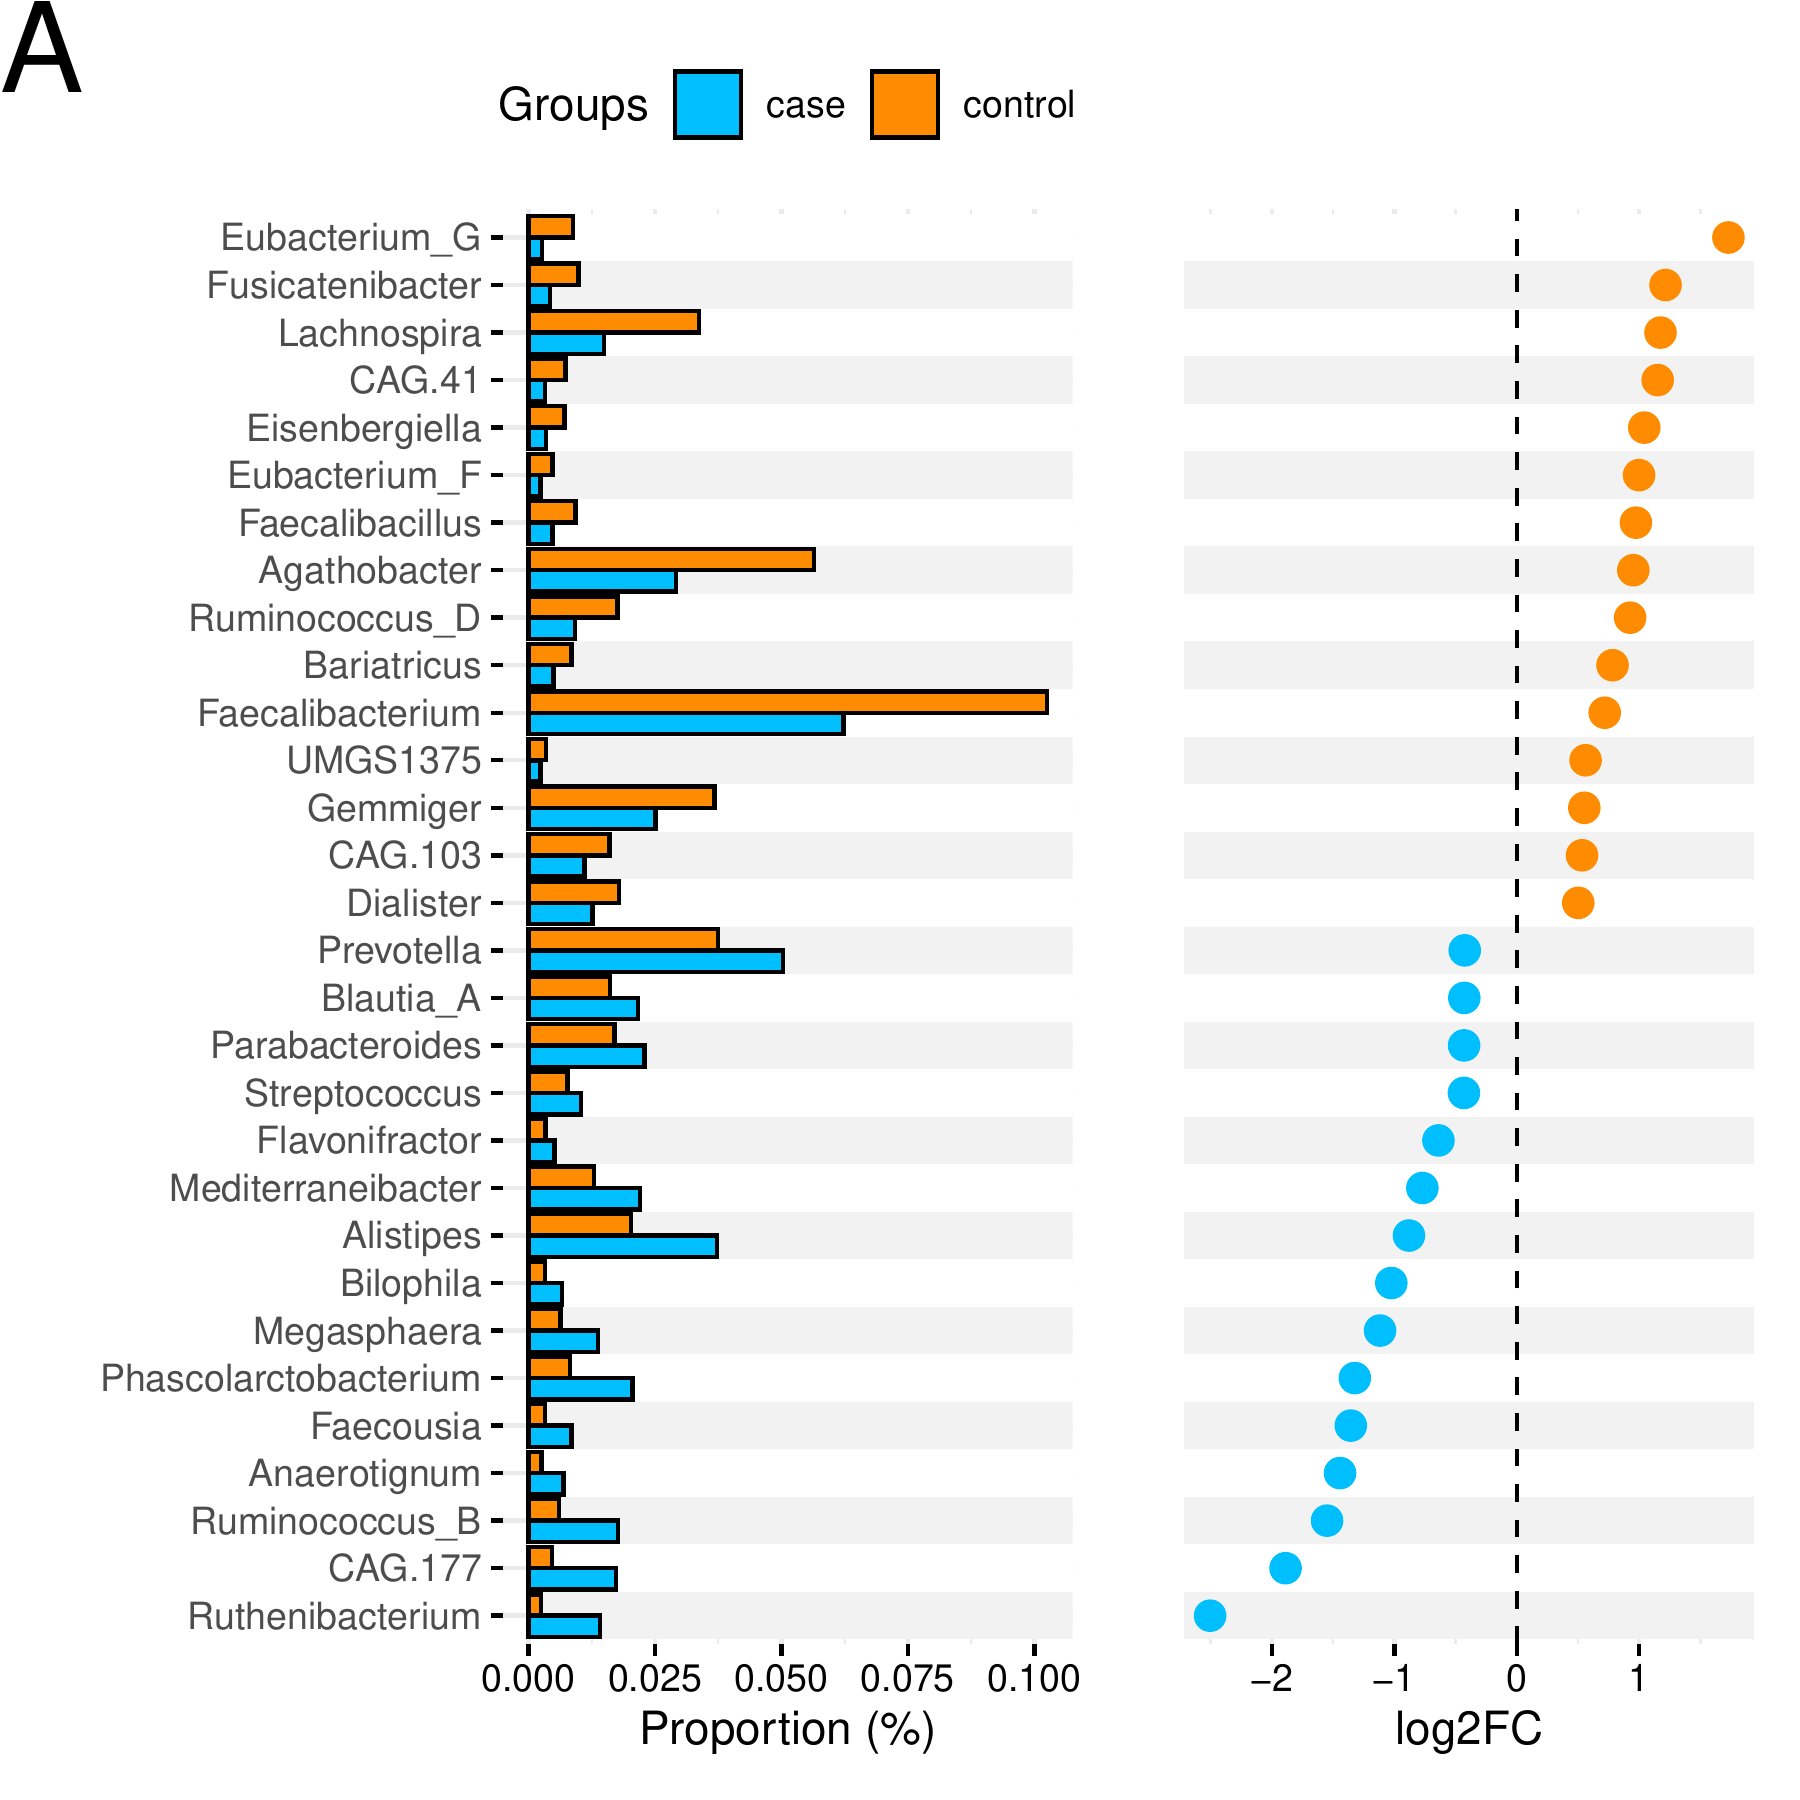
\includegraphics[width=0.5\textwidth,height=0.5\textheight]{../../Analysis_shotgun_ERP012177/04_Wilcoxon/atlas/output/class_ERP012177_pvalue0.05case_control_metagenomics.png}
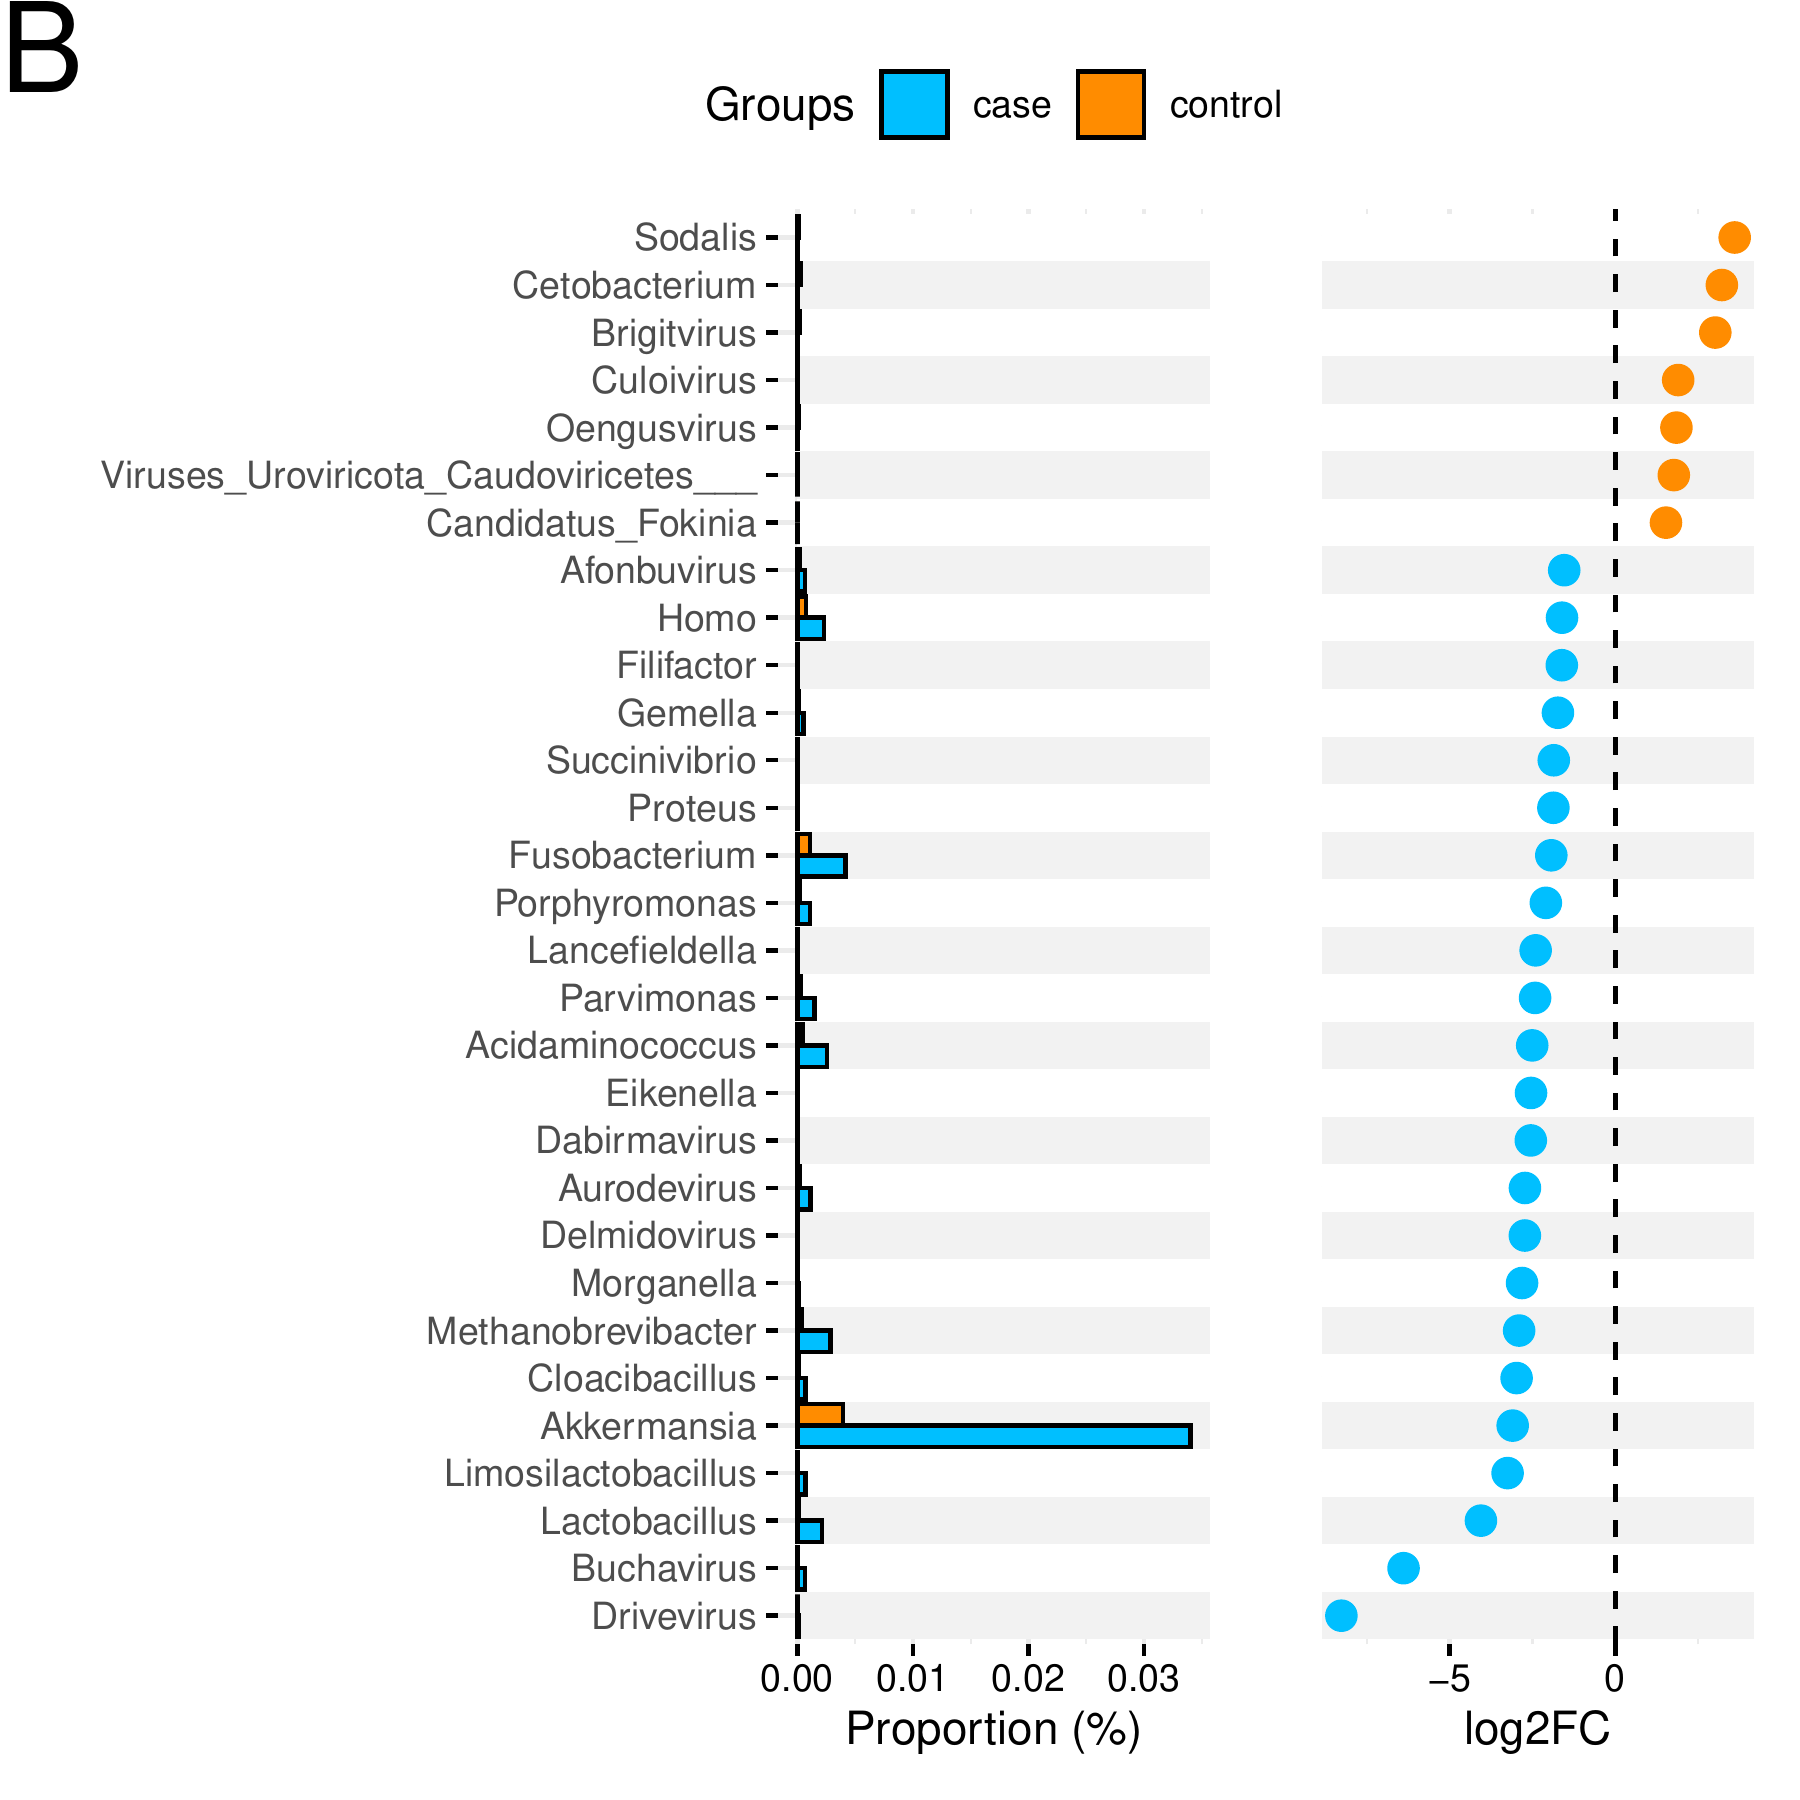
\includegraphics[width=0.5\textwidth,height=0.5\textheight]{../../Analysis_shotgun_ERP012177/04_Wilcoxon/Kraken2/output/class_ERP012177_pvalue0.05case_control_metagenomics.png}

\hypertarget{prjdb4176-1}{%
\subsection{PRJDB4176}\label{prjdb4176-1}}

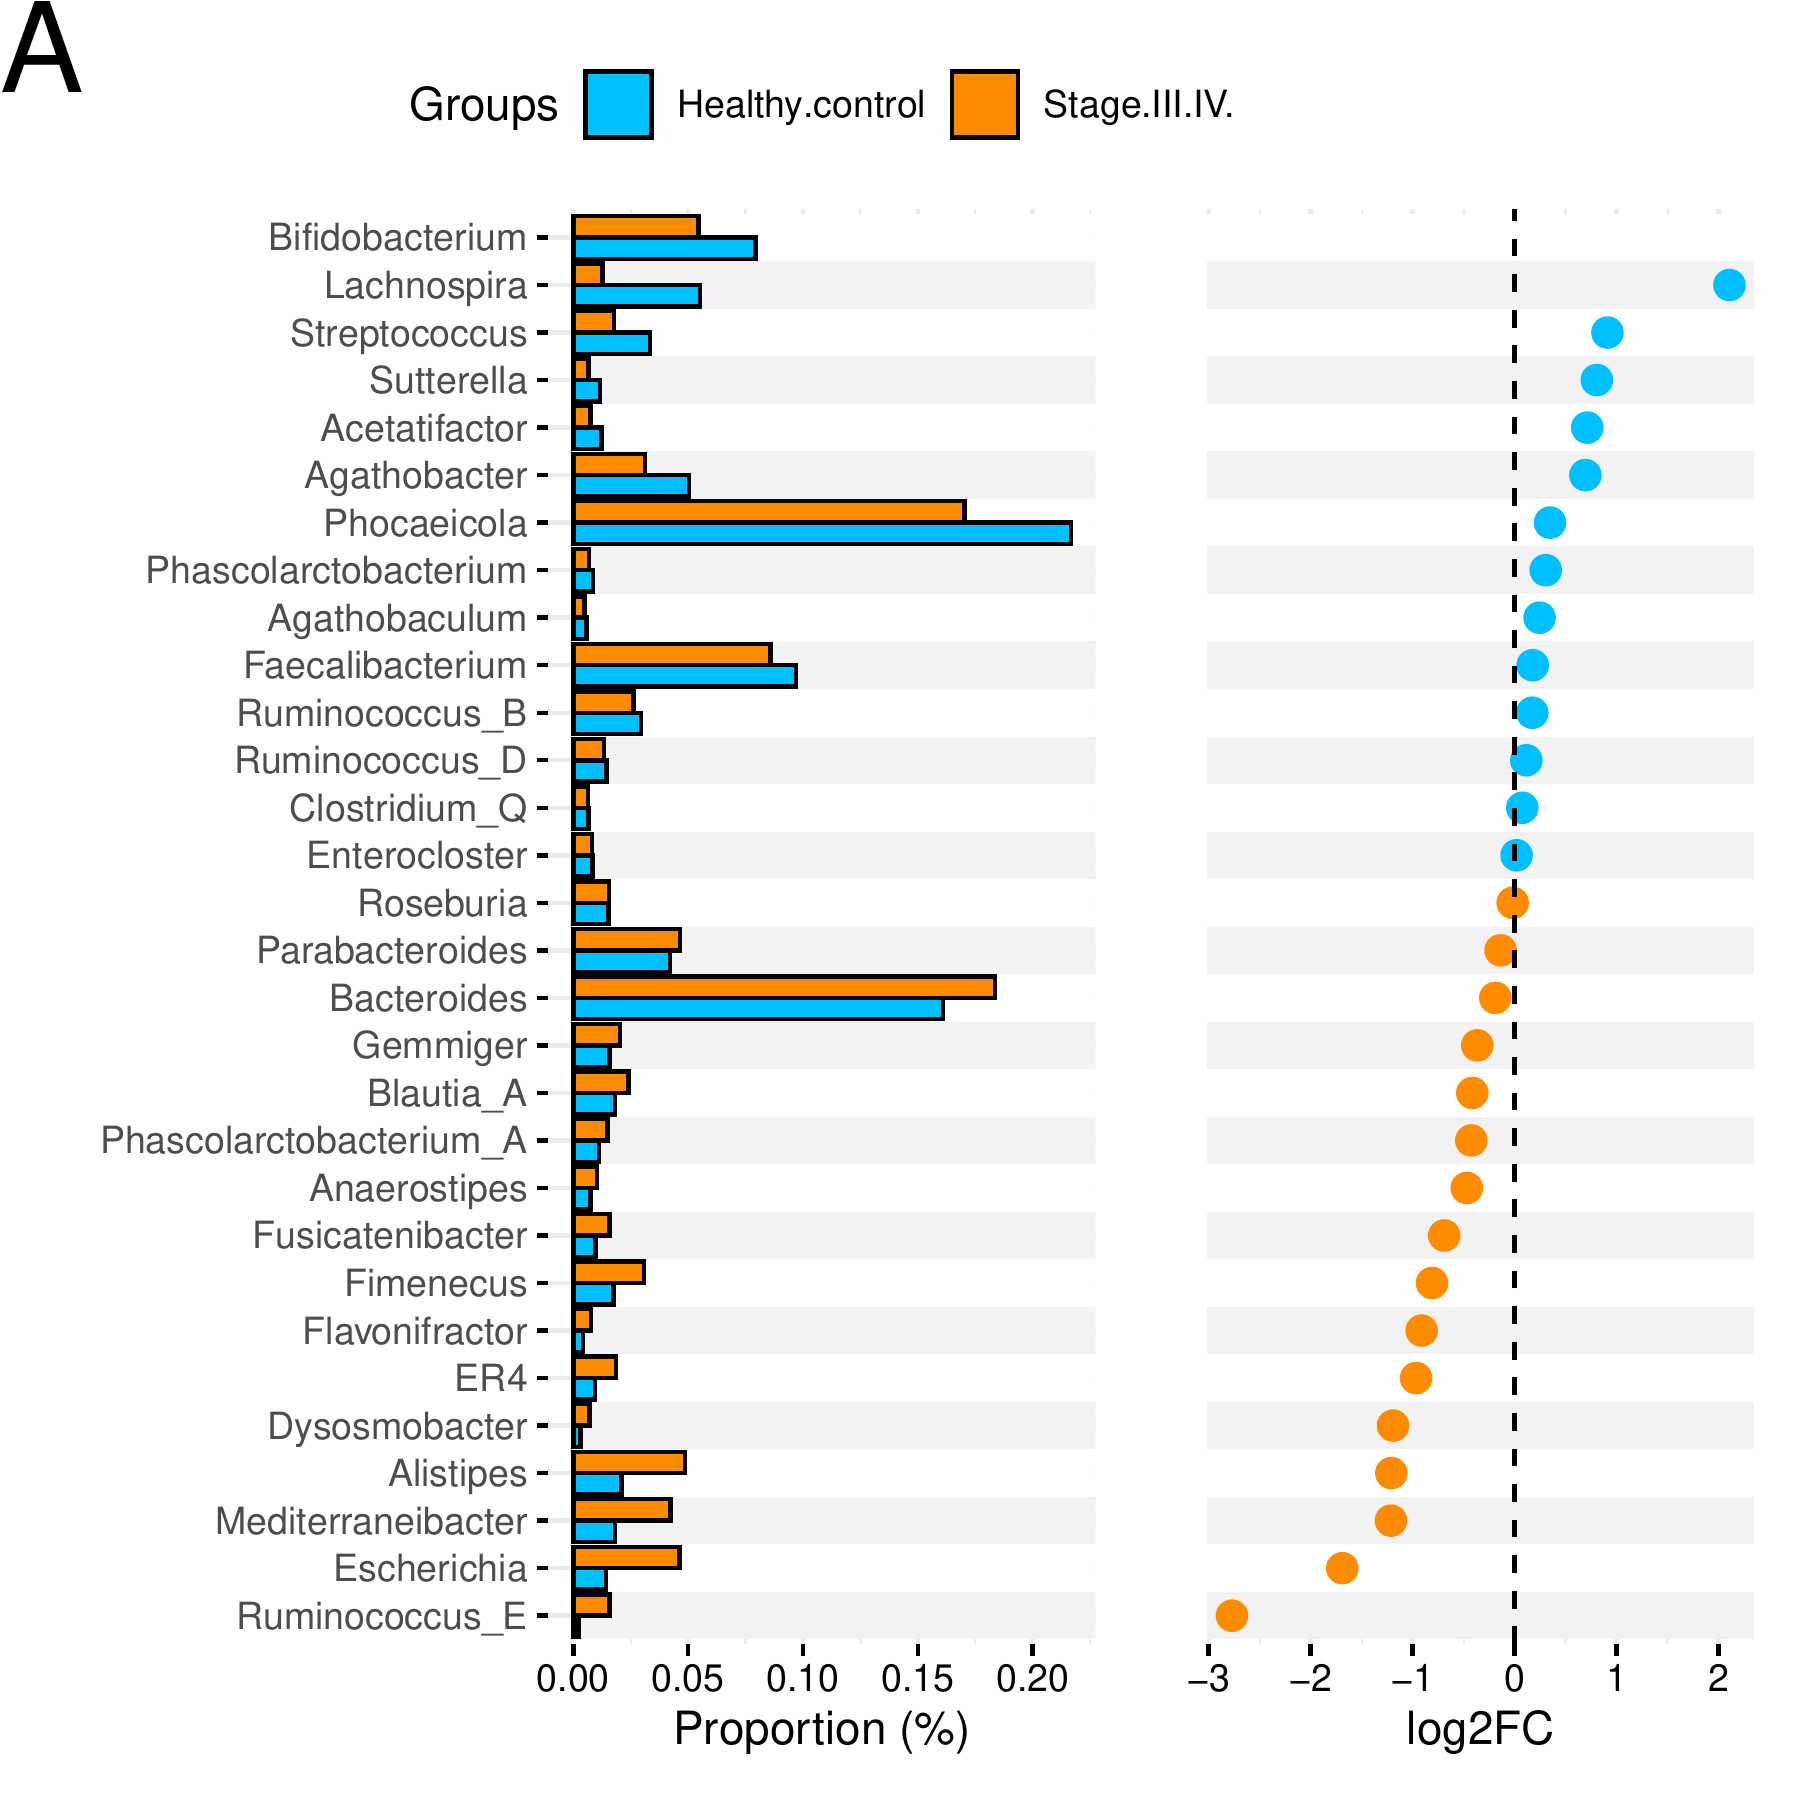
\includegraphics[width=0.5\textwidth,height=0.5\textheight]{../../Analysis_shotgun_PRJDB4176/04_Wilcoxon/atlas/output/class_PRJDB4176_pvalue0.05Stage.III.IV._Healthy.control_metagenomics.png}
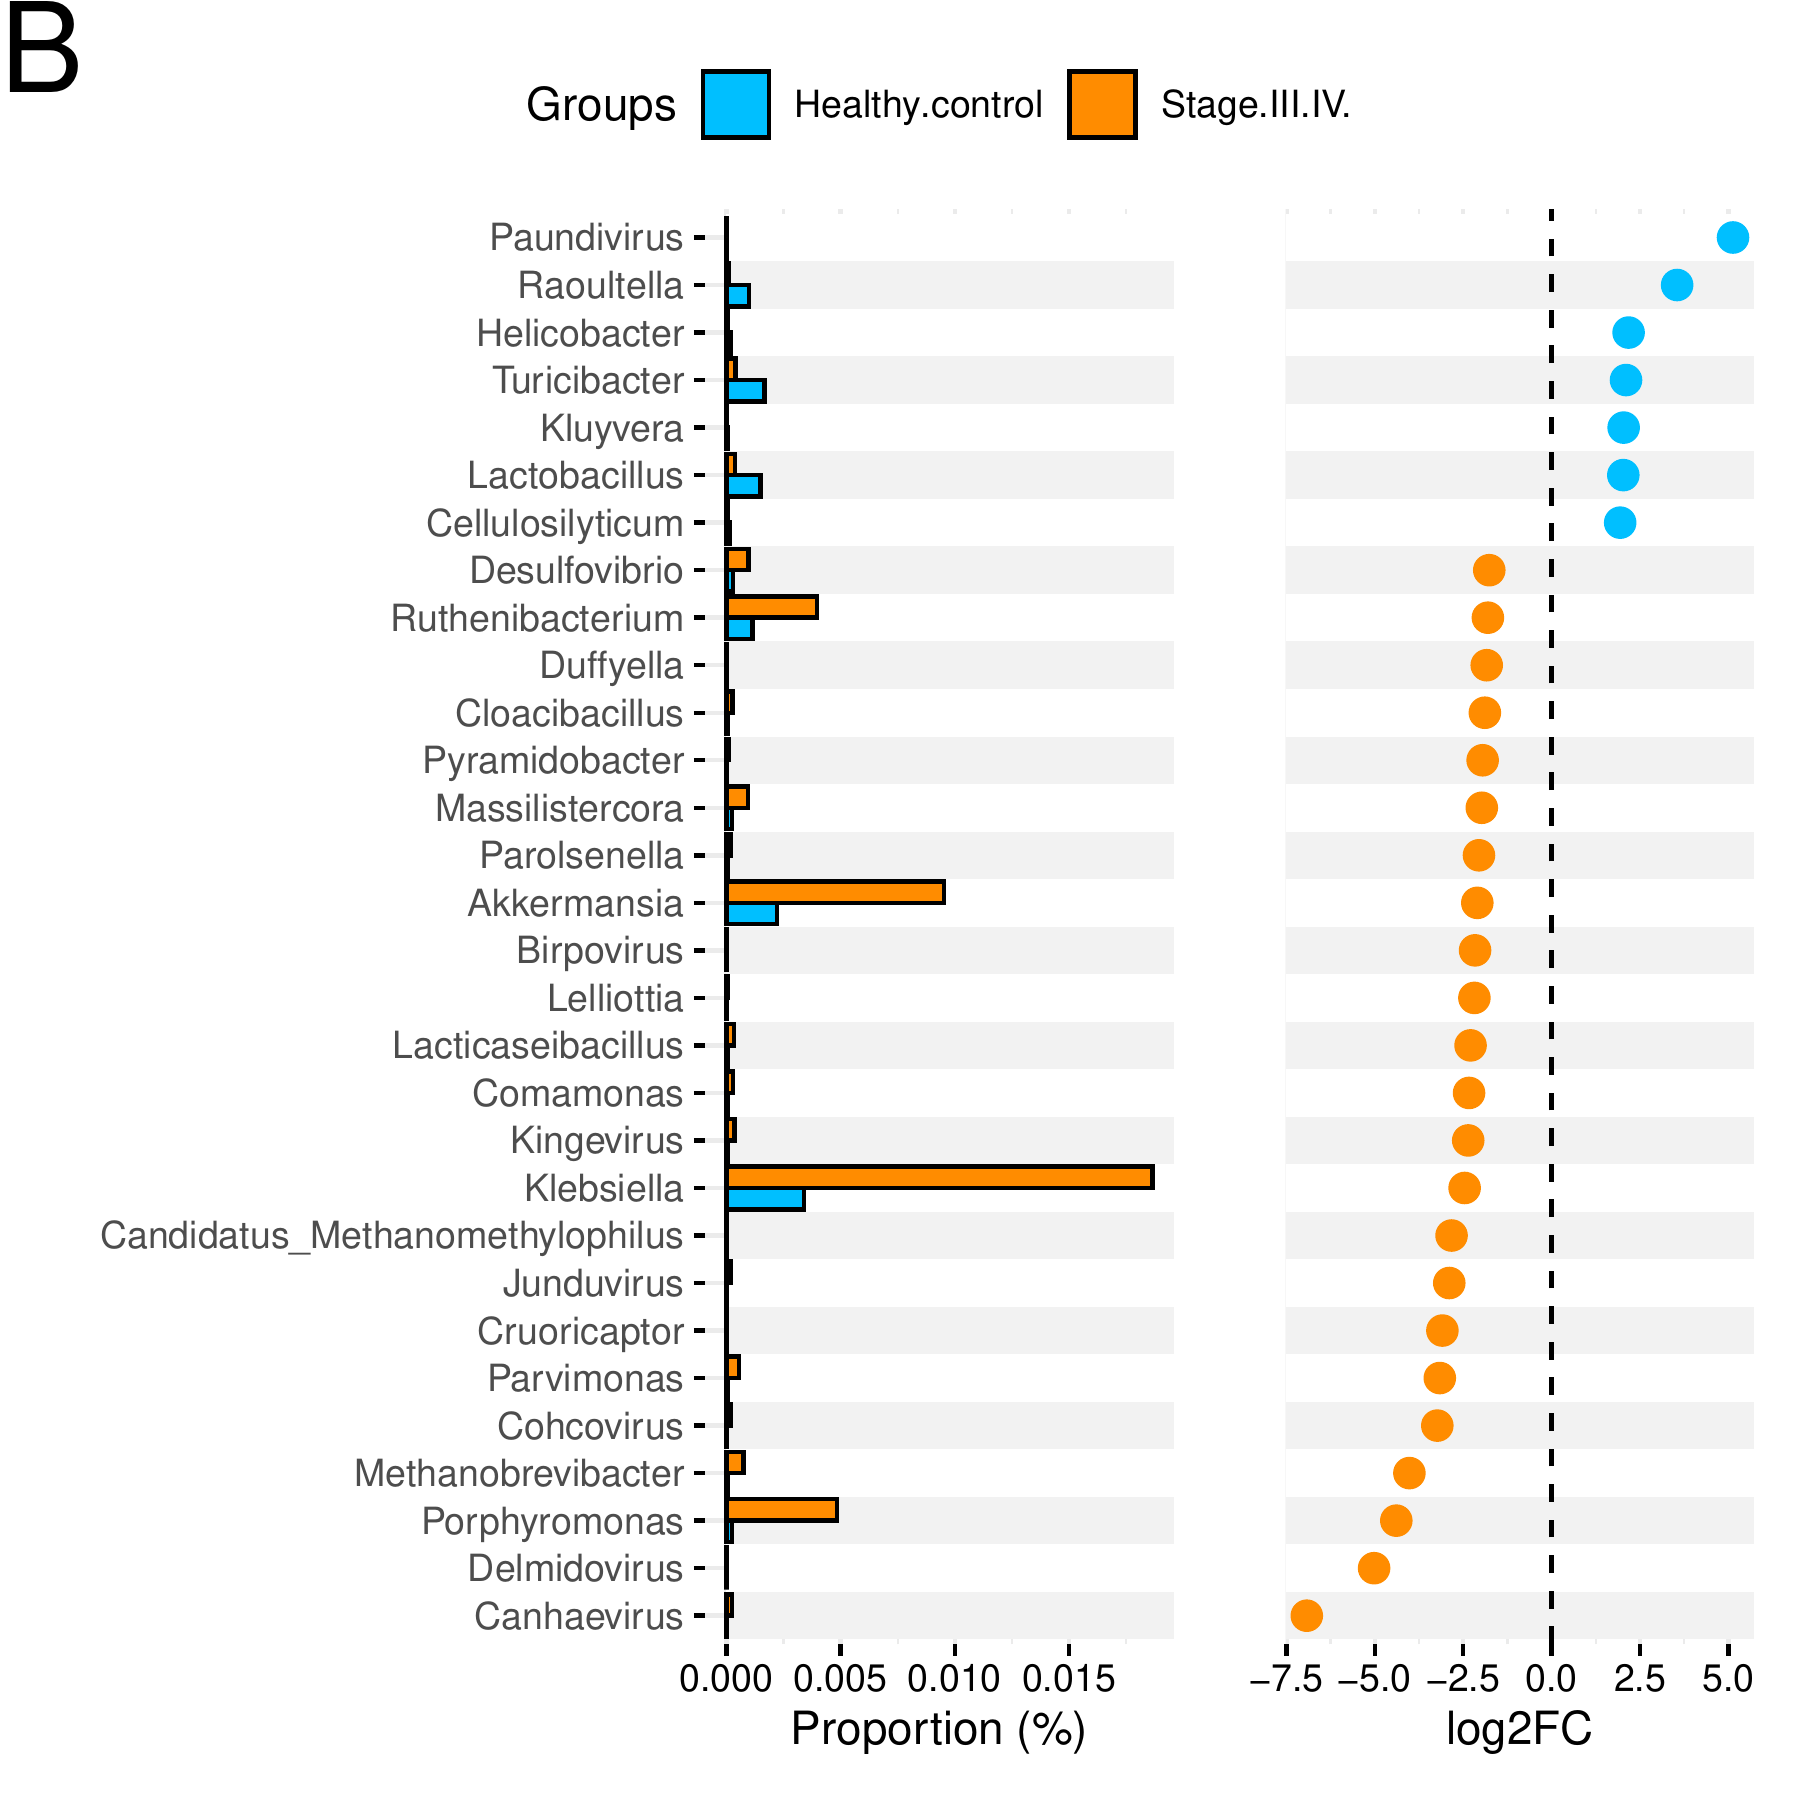
\includegraphics[width=0.5\textwidth,height=0.5\textheight]{../../Analysis_shotgun_PRJDB4176/04_Wilcoxon/Kraken2/output/class_PRJDB4176_pvalue0.05Stage.III.IV._Healthy.control_metagenomics.png}

\hypertarget{figure4-venny}{%
\section{Figure4 Venny}\label{figure4-venny}}

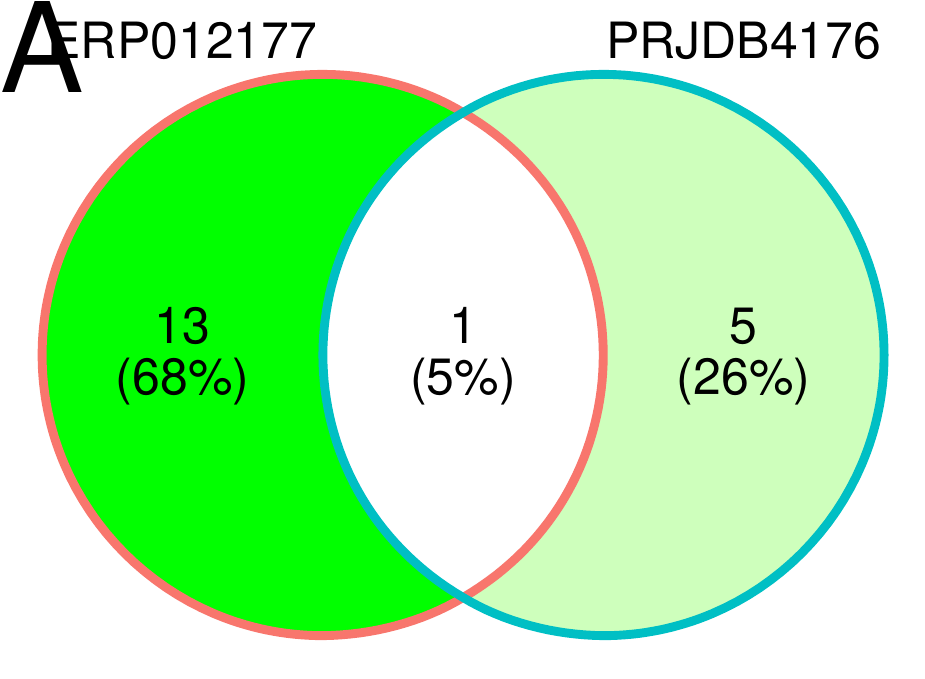
\includegraphics[width=0.5\textwidth,height=0.5\textheight]{../../Venny/Atlas_wilcox_venny.png}
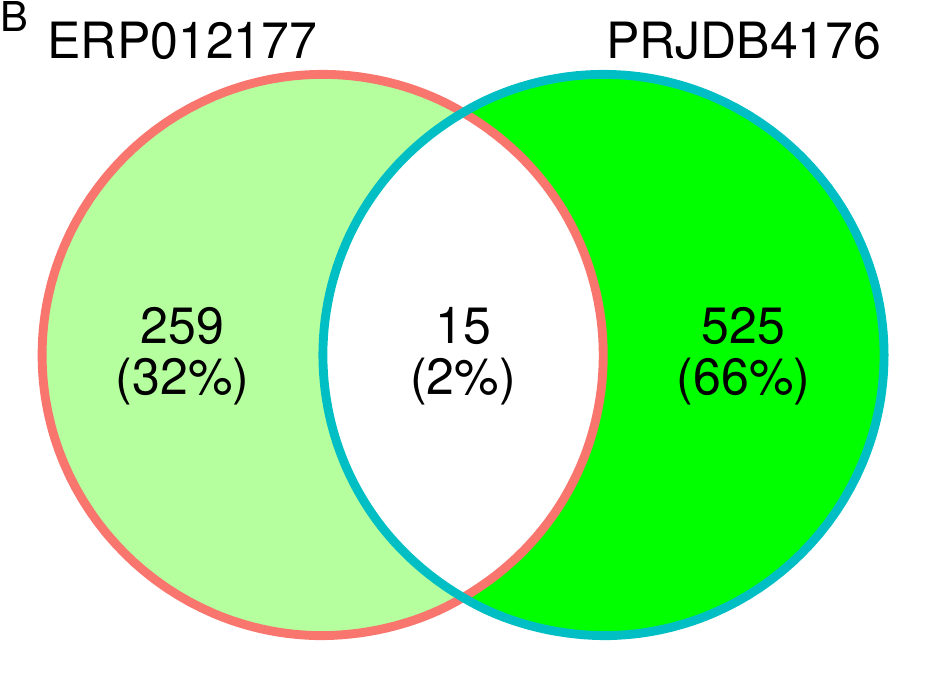
\includegraphics[width=0.5\textwidth,height=0.5\textheight]{../../Venny/Kraken2_wilcox_venny.png}

References:

{[}1{]} Zeller G, et al.~Potential of fecal microbiota for early‐stage
detection of colorectal cancer. Mol Syst Biol. 2014;10:766.

{[}2{]} Jovel J, et al.~Characterization of the gut microbiome using 16S
or shotgun metagenomics. Front Microbiol. 2016;7:459.

{[}3{]} Yachida S, et al.~Metagenomic and metabolomic analyses reveal
distinct stage-specific phenotypes of the gut microbiota in colorectal
cancer. Nat Med. 2019;25:968-76.

{[}4{]} Lindgreen S, et al.~An evaluation of the accuracy and speed of
metagenome analysis tools. Sci Rep.~2016;6:19233.

{[}5{]} Wirbel J, et al.~Meta-analysis of fecal metagenomes reveals
global microbial signatures that are specific for colorectal cancer. Nat
Med. 2019;25:679-89.

{[}6{]} Thomas AM, et al.~Metagenomic analysis of colorectal cancer
datasets identifies cross-cohort microbial diagnostic signatures and a
link with choline degradation. Nat Med. 2019;25:667-78.

{[}7{]} Flemer B, et al.~Tumour-associated and non-tumour-associated
microbiota in colorectal cancer. Gut. 2017;66:633-43.

{[}8{]} Gao R, et al.~Colorectal cancer-associated microbiota
contributes to oncogenic epigenetic signatures. Nat Commun.
2019;10:4285.

{[}9{]} Zitvogel L, et al.~The microbiome in cancer immunotherapy:
Diagnostic tools and therapeutic strategies. Science. 2018;359:1366-70.

{[}10{]} Nayfach S, et al.~New insights from uncultivated genomes of the
global human gut microbiome. Nature. 2019;568:505-10.

{[}11{]} Wood DE, Salzberg SL. Kraken: ultrafast metagenomic sequence
classification using exact alignments. Genome Biol. 2014;15:R46.

{[}12{]} McMurdie PJ, Holmes S. phyloseq: an R package for reproducible
interactive analysis and graphics of microbiome census data. PLoS One.
2013;8:e61217.

{[}13{]} Wright MN, Ziegler A. ranger: A Fast Implementation of Random
Forests for High Dimensional Data in C++ and R. J Stat Softw.
2017;77:1-17.

{[}14{]} Kuhn M. Building predictive models in R using the caret
package. J Stat Softw. 2008;28:1-26.

{[}15{]} Derrac J, et al.~A practical tutorial on the use of
nonparametric statistical tests as a methodology for comparing
evolutionary and swarm intelligence algorithms. Swarm Evol Comput.
2011;1:3-18.

\end{document}
